\documentclass[12pt, a4paper]{article}
\usepackage[spanish]{babel}
\usepackage[utf8]{inputenc}
\usepackage{lmodern}
\usepackage{fancyhdr}
\usepackage{graphicx}
\usepackage{hyperref}
\usepackage{titlesec}
\usepackage{enumitem}
\usepackage{amsfonts}
\usepackage{amssymb}
\usepackage{xcolor}
\usepackage{float}
\usepackage{listings}
\usepackage{tcolorbox}
\usepackage{booktabs}
\usepackage{longtable}
\usepackage{geometry}
\usepackage{mathtools}

% Margenes
\geometry{
    left=2.5cm,
    right=2.5cm,
    top=2.5cm,
    bottom=2.5cm
}

% Colores
\definecolor{azul}{RGB}{0, 51, 102}
\definecolor{gris}{RGB}{245, 245, 245}

\setlength{\parindent}{0pt}
\setlength{\parskip}{10pt}
\pagestyle{fancy}
\fancyhf{}
\renewcommand{\headrulewidth}{0pt}
\fancyfoot[C]{\thepage}

\begin{document}

    \begin{center}
        {\Huge \textcolor{azul}{\textbf{Bitácora de Pasantías}}}

        \vspace{0.5cm}

        {\Large Lorena Rojas}

        {\large The Factory HKA}

        \vspace{1cm}

        {\large 19 de Enero - 29 de Mayo}
    \end{center}

    \section*{Fecha: 19/01/2026}

    \subsection*{Actividades}

    \begin{itemize}
        \item Conocer la interfaz de desarrollo del firmware para el ESP32
        \item Insvestigar acerca de librerias MQTT para ESP32
    \end{itemize}

    \subsection*{Aprendizajes}

    MQTT es un protocolo de mensajería ligero para IoT con un modelo de publicación/suscripción que ofrece una comunicación fiable en tiempo real con un consumo mínimo de código y ancho de banda. Resulta especialmente beneficioso para dispositivos con recursos limitados y redes con bajo ancho de banda, lo que lo ha convertido en un protocolo ampliamente adoptado en los sectores de IoT, internet móvil, IoV y energía.

    El ESP32 , una versión mejorada del ESP8266 , es un microcontrolador de bajo coste y bajo consumo en un chip (SOM). Además del módulo Wi-Fi, el ESP32 también incluye un módulo Bluetooth 4.0. La CPU de doble núcleo opera a una frecuencia de 80 a 240 MHz. Contiene dos módulos Wi-Fi y Bluetooth, y varios pines de entrada y salida. El ESP32 es ideal para proyectos de IoT.

    El uso de MQTT en ESP32 ofrece varias ventajas:

    \begin{itemize}
        \item En primer lugar, MQTT es un protocolo de mensajería liviano optimizado para dispositivos y redes restringidos como ESP32 y Wi-Fi, por lo que tiene un impacto mínimo en la energía y el ancho de banda.
        \item En segundo lugar, MQTT admite diferentes niveles de confiabilidad y calidad de servicio para adaptarse a las capacidades de ESP32. Esta flexibilidad lo hace ideal incluso en redes inestables.
        \item En tercer lugar, ESP32 y MQTT se utilizan ampliamente en aplicaciones de IoT, lo que permite una buena integración con las soluciones de IoT. El protocolo MQTT también está diseñado para simplificar la integración con plataformas en la nube y permitir el control de dispositivos y la monitorización de datos en redes.
    \end{itemize}

    {\color{red} \subsubsection*{Instalación de VS con MinGW}}

    Logré crear y compilar un archivo programado en C a traves de Visual Studio Code, y sin necesidad de modificar la PATH del sistema. Se logró configurando la extensión de C/C++ desde el VS mediante el siguiente cambio a la PATH:

    \begin{verbatim}
                "C:/esp/tools/Espressif/**",
                "C:/esp/esp-idf-v5.5.2/**"
    \end{verbatim}

    \subsection*{Dificultades}

    No se ha podido compilar un proyecto "get-started" de ESP32 desde el Visual Studio Code, se sigue intentando... El problema esta en que el computador no lee el puerto serial de nuestro ESP32.

    \subsection*{Notas}

    Probar ESP32 en mi computador personal, si tampoco funciona notificar al Ing. Pablo acerca del percanse con el dispositivo.

    \section*{Fecha: 20/01/2026}

    \subsection*{Actividades}

    \begin{itemize}
        \item Realización de mini-proyecto con ESP32 y MQTT
        \item Posible reunión con Eder y Pablo para definir y/o establecer funcionalidades
        \item (OPCIONAL) Revisar la interfaz de desarrollo del I-Smart
    \end{itemize}

    \subsection*{Aprendizajes}

    {\color{red} \subsubsection*{Tarjeta de desarrollo EPS32 DeVKitc V4}}

    \begin{figure} [H]
        \centering
        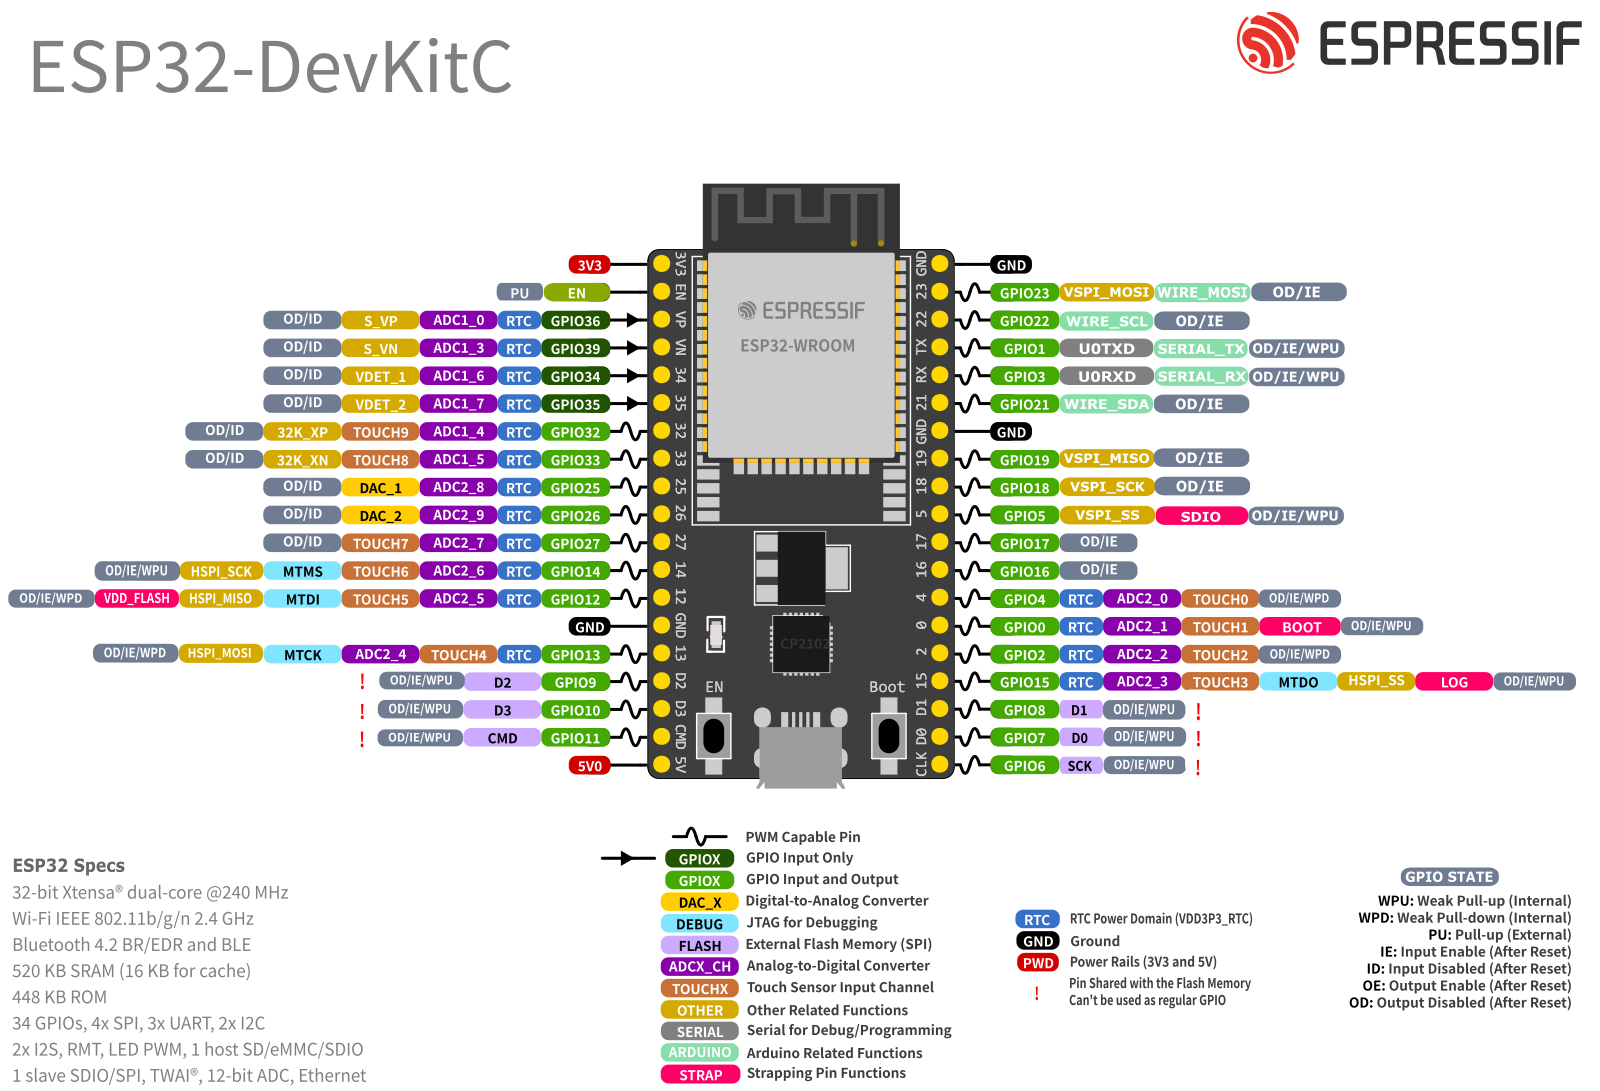
\includegraphics[width=0.9\linewidth]{Img/esp32_devkitC_v4_pinlayout.png}
        \label{fig:placeholder}
    \end{figure}
    

    {\color{red} \subsubsection*{Ventajas que ofrece el protocolo MQTT para la escalabilidad y eficiencia en proyectos IoT}}

    El protocolo MQTT (MQ Telemetry Transport) ofrece diversas ventajas diseñadas específicamente para optimizar la escalabilidad y la eficiencia en proyectos de Internet de las Cosas (IoT):

    \begin{itemize}
        \item \textbf{Ligereza y bajo consumo de recursos:} Una de las principales fortalezas de este protocolo es su ligereza, lo que lo hace perfecto para ser implementado en dispositivos muy pequeños que cuentan con recursos limitados. Esta eficiencia se traduce en un bajo consumo de recursos del sistema, permitiendo que dispositivos sencillos se comuniquen a través de Internet de forma simple.
        \item \textbf{Capacidad de escalabilidad masiva:} MQTT permite la escalabilidad necesaria para conectar millones de dispositivos a la vez. Esto facilita el manejo de grandes grupos de dispositivos siendo la opción correcta para este proyecto.
        \item \textbf{Arquitectura basada en tópicos y un broker:} El funcionamiento de MQTT se basa en tópicos, que actúan como canales de información a los que los clientes pueden suscribirse o en los que pueden publicar. El broker actúa como el administrador central, encargándose de que la información llegue a su destino y permitiendo que varios dispositivos estén conectados a un mismo tópico simultáneamente,.
        \item \textbf{Niveles de Calidad de Servicio (QoS):} Para asegurar la eficiencia en la entrega de mensajes, el protocolo ofrece tres niveles de servicio:
        \begin{itemize}
            \item \textbf{Nivel 0:} El mensaje se envía una vez sin confirmar recepción.
            \item \textbf{Nivel 1:} Se garantiza que el mensaje se entregue al menos una vez.
            \item \textbf{Nivel 2:} Se garantiza que el mensaje se entregue exactamente una vez, evitando duplicados.
        \end{itemize}
        \item \textbf{Optimización del tráfico de datos:} En las aplicaciones de IoT, no siempre es necesario enviar datos en cada instante; el uso de intervalos (como cada 5 segundos) ayuda a mantener la eficiencia de la red y del dispositivo. Además, el uso de \textbf{brokers avanzados} permite realizar funciones como el filtrado de información y la creación de bases de datos para gestionar mejor el flujo de mensajes.
    \end{itemize}

    {\color{red} \subsubsection*{Conexiones cliente-agente MQTT}}
    MQTT utiliza TCP/IP para conectarse al broker.
    
    TCP es un protocolo orientado a conexión con corrección de errores y garantiza que los paquetes se reciban en orden.
    
    Se puede considerar que una conexión TCP/IP es similar a una conexión telefónica .
    
    Una vez que se establece una conexión telefónica, puede hablar hasta que una de las partes cuelgue .
    
    La mayoría de los clientes MQTT se conectarán al broker y permanecerán conectados incluso si no están enviando datos.
    
    Las conexiones son reconocidas por el broker mediante un mensaje de reconocimiento de conexión .

    \begin{figure} [H]
        \centering
        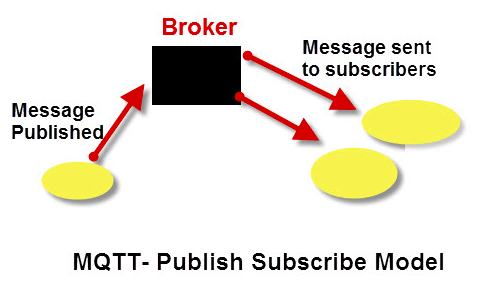
\includegraphics[width=0.6\linewidth]{Img/image2.png}
        \label{fig:placeholder}
    \end{figure}

    \subsection*{Dificultades}

    Tuve que realizar una tardada investigacion sobre MQTT para comprender su uso en ESP-IDF. A mitad de la tarde es que pude comenzar con mi proyecto de MQTT.

    Mantengo dificultades de compilacion en el Visual Studio Code.

    \subsection*{Notas}

    Se propone el uso de MQTT sobre WebSockets con \textbf{Mosquitto}, esto por que es un broker de codigo abierto, gratis y el mas utilizado en MQTT.

    Se aumento el repertorio de documentacion en el cuaderno de NotebookLM.

    Se inicio un proyecto para probar el ESP32 con MQTT y el Broker Mosquitto, falta trabajar en eso (se buscara concluir mañana).

    \section*{Fecha: 21/01/2026}

    \subsection*{Actividades}

    \begin{itemize}
        \item Terminar Mini-Proyecto con MQTT y mosquitto
        \item Poner a prueba la base de datos de mosquitto
        \item Definir funcionalidades principales a obtener
    \end{itemize}

    \subsection*{Aprendizajes}

    El código de error 201 es: en el ecosistema de Espressif, \texttt{WIFI\_REASON\_NO\_AP\_FOUND}. Esto significa que el ESP32 no está viendo ninguna red con el nombre "LorenaWiFi". Es un problema de visibilidad.

    Los errores de compilación no está realmente en el archivo JSON (ese archivo es solo para que VS Code no marque errores en rojo), sino en el sistema de construcción CMake de ESP-IDF. En ESP-IDF, para mantener el binario pequeño, el compilador no incluye todas las librerías automáticamente. Se tiene que declarar explícitamente al proyecto. Por ejemplo, en mi caso, tuve que editar el archivo \texttt{CMakeLists.txt} que está dentro de la carpeta main, tal que:

    \begin{verbatim}
        idf_component_register(SRCS "station_example_main.c"
                    PRIV_REQUIRES esp_wifi nvs_flash
                    INCLUDE_DIRS "."
                    REQUIRES esp_http_client esp_event)
    \end{verbatim}

    Se empleo el protocolo de comunicacion HTTP a partir del ESP32, para esto se partio del codigo base suministrado por Espressif en \texttt{protocolos}/\texttt{esp\_http\_client}:

    \begin{verbatim}
        esp_http_client_config_t config = {
            .host = CONFIG_EXAMPLE_HTTP_ENDPOINT,
            .path = "/get",
            .query = "esp",
            .event_handler = _http_event_handler,
            .user_data = local_response_buffer,        // Pass address of local buffer to get response
            .disable_auto_redirect = true,
        };
        ESP_LOGI(TAG, "HTTP request with url =>");
        esp_http_client_handle_t client = esp_http_client_init(&config);
    
        // GET
        esp_err_t err = esp_http_client_perform(client);
        if (err == ESP_OK) {
            ESP_LOGI(TAG, "HTTP GET Status = %d, content_length = %"PRId64,
                    esp_http_client_get_status_code(client),
                    esp_http_client_get_content_length(client));
        } else {
            ESP_LOGE(TAG, "HTTP GET request failed: %s", esp_err_to_name(err));
        }
        ESP_LOG_BUFFER_HEX(TAG, local_response_buffer, strlen(local_response_buffer));
    \end{verbatim}

    El cual se adaptó de la siguiente forma, con el fin de enviar datos a una pagina Open Source \textit{ThingsSpeak}:

    \begin{verbatim}
        esp_http_client_config_t config = {
            .url = url,
            .method = HTTP_METHOD_GET,
        };
        esp_http_client_handle_t client = esp_http_client_init(&config);
    
        // GET
        esp_err_t err = esp_http_client_perform(client);
        if (err == ESP_OK) {
            ESP_LOGI(TAG, "HTTP GET Status = %d, content_length = %"PRId64,
                    esp_http_client_get_status_code(client),
                    esp_http_client_get_content_length(client));
        } else {
            ESP_LOGE(TAG, "HTTP GET request failed: %s", esp_err_to_name(err));
        }
    
        esp_http_client_cleanup(client);
    \end{verbatim}

    Con estos cambios se logro satisfactoriamente la visualizacion de datos en la web, sentando las bases para avanzar y transformar el proyecto a un protocolo MQTT mediante \texttt{mosquitto}.

    Con mosquitto, se pudo crear un servidor local MQTT teniendo como host el computador personal, siendo el codigo base el siguiente:

    \begin{verbatim}
        static void mqtt_event_handler(void *handler_args, esp_event_base_t base, int32_t event_id, void *event_data)
        {
            ESP_LOGD(TAG, "Event dispatched from event loop base=%s, event_id=%" PRIi32, base, event_id);
            esp_mqtt_event_handle_t event = event_data;
            esp_mqtt_client_handle_t client = event->client;
            int msg_id;
            switch ((esp_mqtt_event_id_t)event_id) {
            case MQTT_EVENT_CONNECTED:
                ESP_LOGI(TAG, "MQTT_EVENT_CONNECTED");
                msg_id = esp_mqtt_client_subscribe(client, "/topic/qos0", 0);
                ESP_LOGI(TAG, "sent subscribe successful, msg_id=%d", msg_id);
        
                msg_id = esp_mqtt_client_subscribe(client, "/topic/qos1", 1);
                ESP_LOGI(TAG, "sent subscribe successful, msg_id=%d", msg_id);
        
                msg_id = esp_mqtt_client_unsubscribe(client, "/topic/qos1");
                ESP_LOGI(TAG, "sent unsubscribe successful, msg_id=%d", msg_id);
                break;
            case MQTT_EVENT_DISCONNECTED:
                ESP_LOGI(TAG, "MQTT_EVENT_DISCONNECTED");
                break;
        
            case MQTT_EVENT_SUBSCRIBED:
                ESP_LOGI(TAG, "MQTT_EVENT_SUBSCRIBED, msg_id=%d", event->msg_id);
                msg_id = esp_mqtt_client_publish(client, "/topic/qos0", "data", 0, 0, 0);
                ESP_LOGI(TAG, "sent publish successful, msg_id=%d", msg_id);
                break;
            case MQTT_EVENT_UNSUBSCRIBED:
                ESP_LOGI(TAG, "MQTT_EVENT_UNSUBSCRIBED, msg_id=%d", event->msg_id);
                break;
            case MQTT_EVENT_PUBLISHED:
                ESP_LOGI(TAG, "MQTT_EVENT_PUBLISHED, msg_id=%d", event->msg_id);
                break;
            case MQTT_EVENT_DATA:
                ESP_LOGI(TAG, "MQTT_EVENT_DATA");
                printf("TOPIC=%.*s\r\n", event->topic_len, event->topic);
                printf("DATA=%.*s\r\n", event->data_len, event->data);
                if (strncmp(event->data, "send binary please", event->data_len) == 0) {
                    ESP_LOGI(TAG, "Sending the binary");
                    send_binary(client);
                }
                break;
            case MQTT_EVENT_ERROR:
                ESP_LOGI(TAG, "MQTT_EVENT_ERROR");
                if (event->error_handle->error_type == MQTT_ERROR_TYPE_TCP_TRANSPORT) {
                    ESP_LOGI(TAG, "Last error code reported from esp-tls: 0x%x", event->error_handle->esp_tls_last_esp_err);
                    ESP_LOGI(TAG, "Last tls stack error number: 0x%x", event->error_handle->esp_tls_stack_err);
                    ESP_LOGI(TAG, "Last captured errno : %d (%s)",  event->error_handle->esp_transport_sock_errno,
                             strerror(event->error_handle->esp_transport_sock_errno));
                } else if (event->error_handle->error_type == MQTT_ERROR_TYPE_CONNECTION_REFUSED) {
                    ESP_LOGI(TAG, "Connection refused error: 0x%x", event->error_handle->connect_return_code);
                } else {
                    ESP_LOGW(TAG, "Unknown error type: 0x%x", event->error_handle->error_type);
                }
                break;
            default:
                ESP_LOGI(TAG, "Other event id:%d", event->event_id);
                break;
            }
        }
        
        static void mqtt_app_start(void)
        {
            const esp_mqtt_client_config_t mqtt_cfg = {
                .broker = {
                    .address.uri = CONFIG_BROKER_URI,
                    .verification.certificate = (const char *)mqtt_eclipseprojects_io_pem_start
                },
            };
        
            ESP_LOGI(TAG, "[APP] Free memory: %" PRIu32 " bytes", 
                    esp_get_free_heap_size());
            esp_mqtt_client_handle_t client = esp_mqtt_client_init(&mqtt_cfg);
            /* The last argument may be used to pass data to the event handler, in this example mqtt_event_handler */
            esp_mqtt_client_register_event(client, ESP_EVENT_ANY_ID, 
                                            mqtt_event_handler, NULL);
            esp_mqtt_client_start(client);
        }
    \end{verbatim}

    El cual se modifico de la siguiente forma:

    \begin{verbatim}
        static void mqtt_event_handler(void *handler_args, 
        esp_event_base_t base, int32_t event_id, void *event_data)
        {
            ESP_LOGD(TAG, "Event dispatched from event loop base=%s, 
                    event_id=%" PRIi32, base, event_id);
            esp_mqtt_event_handle_t event = event_data;
            esp_mqtt_client_handle_t client = event->client;
            switch ((esp_mqtt_event_id_t)event_id) {
            case MQTT_EVENT_CONNECTED:
                ESP_LOGI(TAG, "MQTT_EVENT_CONNECTED");
                //msg_id = esp_mqtt_client_subscribe(client, "pruebahka/lorena1", 0);
                //ESP_LOGI(TAG, "sent subscribe successful, msg_id=%d", msg_id);
        
                xTaskCreate(mqtt_publish_task, "mqtt_publish_task", 4096, 
                            NULL, 5, NULL);
                break;
        
            case MQTT_EVENT_DISCONNECTED:
                ESP_LOGI(TAG, "MQTT_EVENT_DISCONNECTED");
                break;
        
            case MQTT_EVENT_SUBSCRIBED:
                ESP_LOGI(TAG, "MQTT_EVENT_SUBSCRIBED, msg_id=%d", event->msg_id);
                break;
        
            case MQTT_EVENT_UNSUBSCRIBED:
                ESP_LOGI(TAG, "MQTT_EVENT_UNSUBSCRIBED, msg_id=%d", event->msg_id);
                break;
        
            case MQTT_EVENT_PUBLISHED:
                ESP_LOGI(TAG, "MQTT_EVENT_PUBLISHED, msg_id=%d", event->msg_id);
                break;
        
            case MQTT_EVENT_DATA:
                ESP_LOGI(TAG, "MQTT_EVENT_DATA");
                printf("TOPIC=%.*s\r\n", event->topic_len, event->topic);
                printf("DATA=%.*s\r\n", event->data_len, event->data);
                break;
        
            case MQTT_EVENT_ERROR:
                ESP_LOGI(TAG, "MQTT_EVENT_ERROR");
                if (event->error_handle->error_type == 
                    MQTT_ERROR_TYPE_TCP_TRANSPORT) {
                    ESP_LOGI(TAG, "Last error code reported from esp-tls: 0x%x", 
                            event->error_handle->esp_tls_last_esp_err);
                    ESP_LOGI(TAG, "Last tls stack error number: 0x%x", 
                            event->error_handle->esp_tls_stack_err);
                    ESP_LOGI(TAG, "Last captured errno : %d (%s)",  
                            event->error_handle->esp_transport_sock_errno,
                             strerror(event->error_handle->esp_transport_sock_errno));
                } else if (event->error_handle->error_type == 
                            MQTT_ERROR_TYPE_CONNECTION_REFUSED) {
                    ESP_LOGI(TAG, "Connection refused error: 0x%x", 
                            event->error_handle->connect_return_code);
                } else {
                    ESP_LOGW(TAG, "Unknown error type: 0x%x", 
                            event->error_handle->error_type);
                }
                break;
        
            default:
                ESP_LOGI(TAG, "Other event id:%d", event->event_id);
                break;
            }
        }
        
        static void mqtt_app_start(void)
        {
            // Es mejor inicializar la estructura a cero primero
            esp_mqtt_client_config_t mqtt_cfg = { 0 }; 
            
            mqtt_cfg.broker.address.hostname = "10.142.223.70";
            mqtt_cfg.broker.address.port = 1883;
            mqtt_cfg.broker.address.transport = MQTT_TRANSPORT_OVER_TCP;
        
            mqtt_cfg.broker.verification.use_global_ca_store = false;
        
            ESP_LOGI(TAG, "Iniciando MQTT hacia el Host: %s", 
                    mqtt_cfg.broker.address.hostname);
            
            esp_mqtt_client_handle_t client = esp_mqtt_client_init(&mqtt_cfg);
            mqttClient = client;
            
            if (client == NULL) {
                ESP_LOGE(TAG, "Error: No se pudo inicializar el cliente 
                        puntero nulo)");
                return;
            }
        
            /* Registrar eventos */
            esp_mqtt_client_register_event(client, ESP_EVENT_ANY_ID, 
                                            mqtt_event_handler, NULL);
            
            /* Iniciar el cliente */
            esp_err_t err = esp_mqtt_client_start(client);
            if (err != ESP_OK) {
                ESP_LOGE(TAG, "Error al iniciar el cliente MQTT: %s", 
                        esp_err_to_name(err));
            }
        }
    \end{verbatim}

    Luego se elavoro una version que envia numeros random desde el ESP32 hacia el broker y de este modo el computador lo recibe conectado al mismo broker. Ya en el computador se elaboro un Scrip en Python que se conecta al mismo broker y recibe la información, de modo que la guarda en un \textit{dataframe} y se genera un archivo CSV que contiene dicha informacion,.siendo este el primer paso para generar una base de datos, que en un futuro se pasara a SQLite.

    \begin{figure} [H]
        \centering
        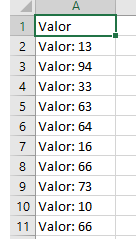
\includegraphics[width=0.3\linewidth]{Img/image1.png}
        \label{fig:placeholder}
    \end{figure}

    \subsection*{Dificultades}

    En vista que el broker con Mosquitto funciona desde un establecimiento puesto localmente, el resultado final se veria afectado por las limitaciones del hardware en cuestion. Por lo tanto, evidentemente se trabajara con un prototipado que maneje solo 100 usuarios mediante el broker de HiveMQ en la nube. 

    \subsection*{Notas}

    Se continuó con el tema de escoger las funcionalidades del proyecto final, para ello se busca responder las siguientes preguntas:

    \begin{itemize}
        \item ¿Qué parámetros específicos de los "datos operativos" son críticos para el monitoreo?

        - Estado
        
        - Errores
        
        - Actividad de impresión

        -
    
        \item ¿Que sensores específicos tiene el equipo fiscal?

        \item En caso de tenerlos, ¿A través de qué sensores específicos del equipo fiscal se realizará la captura?
    
        \item ¿Cómo debe actuar el firmware del ESP32 ante un intento fallido de publicación por MQTT? 
    
        \item ¿Qué mecanismos de diagnóstico y trazabilidad se requieren para registrar el historial de eventos del equipo?
    
        \item ¿Qué alertas específicas debe mostrar la interfaz web o móvil en tiempo real ante un error del equipo fiscal? 
    
        \item ¿Es necesario que el dashboard permita enviar comandos de vuelta al equipo (comunicación bidireccional)?
    
        \item ¿Cómo se deben gestionar y estructurar los datos dentro del servidor MQTT para su posterior consulta?

    \end{itemize}

    Entre otras, se destaca que es lo primordial para una primera version del sistema,

    \begin{enumerate}
        \item Login: Esencial para cumplir con la "comunicación segura".
        \item User Management (Básico): Solo la capacidad de gestionar tu propio usuario y quizás un rol de administrador para las pruebas iniciales de validación.
        \item Device (Add a device): Se necesitara una interfaz para registrar los microcontroladores ESP32 que se conectarán al sistema.
        \item Log capture: Esto se vincula directamente con los "mecanismos de trazabilidad" y la "recolección de datos operativos" (estado, errores, actividad).
        \item System params: Útil para configurar los parámetros de MQTT que el firmware debe utilizar.
        \item Dashboard: Una versión simplificada que muestre los datos operativos capturados desde el equipo fiscal.
        \item Audit logs: Fundamental para la "validación de robustez ante fallos", permitiéndote ver qué pasó si la conexión se perdió.
        \item Firmware Management (Básico): No necesariamente una actualización remota (OTA) compleja aún, sino asegurar que el firmware embebido desarrollado pueda comunicarse con el servidor MQTT.
        \item TLS Certificate: Si buscas una "comunicación segura" desde la primera versión, la gestión de certificados para MQTT es prioritaria.
    \end{enumerate}

    \section*{Fecha: 22/01/2026 (Jueves)} 

    \subsection*{Actividades}

    \begin{itemize}
        \item Descargar Altium
        \item Conseguir interfaz de desarrollo del iSmart
        \item Estudiar interfaz de desarrollo del iSmart
    \end{itemize}

    \subsection*{Aprendizajes}

    Por la razón de ser pasante no será posible tener disposicion de la interfaz iSmart para desarrollo, por lo tanto se seguirá trabajando con el ESP32, buscando similar el estado S1 de una impresora fiscal, por lo menos hasta que se desarrolle el prototipo con el que voy a trabajar.

    En vista de eso, se elaboró la propuesta de otro objetivo para el día: "Conectar ESP32 y Scrip de Python a HiveMQ con MQTTv5". Siendo este un desafio porque presentaba muchos mas protocolos de seguridad, pero cumplia mucho mejor los criterios de la prupuesta donde se especifica que debe ser un sistema seguro.

    \subsection*{Dificultades}

    \subsection*{Notas}

    Para la siguiente semana se buscará diseñar la arquitectura completa de lo que seria el sistema IoT, mientras que en el transcurso del fin de semana se estudiara la documentacion de la impresora fiscal con el fin de trabajar de manera fluida la semana que viene.
    
    \section*{Fecha: 26/01/2026}

    \subsection*{Actividades}

    \begin{itemize}
        \item Leer documentación referente a los protocolos de comunicación en los equipos fiscales
        \item Diseñar arquitectura del sistema IoT
        \item Diseñar arquitectura de comunicaciones MQTT
    \end{itemize}

    \subsection*{Aprendizajes}

    {\color{red} \subsubsection*{Comunicación entre el PC y la impresora fiscal}}

    El protocolo de comunicación de las impresoras fiscales se basa en el estándar RS232 de comunicación serial. Para esto, es necesaria una interfaz de aplicación que gestione este protocolo, esto es, que sea capaz de enviar los comandos desde el computador hacia la impresora e interpretar las respuestas que está retorna. Estos comandos corresponden a protocolos seriales almacenados en el firmware de la impresora.
    
    Los comandos de estos protocolos pueden ser enviados a la impresora de dos maneras: directamente a través del manejo del puerto serial (llamado Protocolo Directo), o utilizando interfaces de programación de aplicaciones (API, Application Programming Interface) las cuales dependen del sistema operativo a utilizar y del lenguaje de programación utilizado para desarrollar el Sistema Administrativo que estará asociado la impresora.

    Los parámetros de configuración del puerto serial son los siguientes:

    \begin{figure}[H]
        \centering
        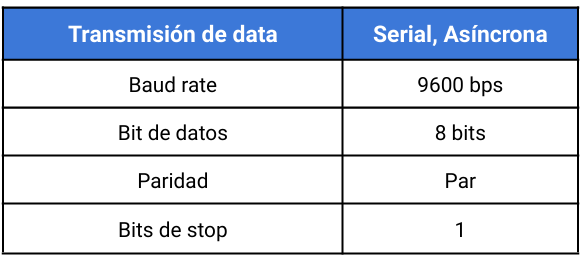
\includegraphics[width=0.7\linewidth]{Img/image.png}
        \label{fig:placeholder}
    \end{figure}

    {\color{red} \subsubsection*{Estructura de la trama de comunicación}}

    La trama de comunicación es el conjunto de datos que debe enviarse a la impresora para que cumpla determinada instrucción; debe enviarse en orden y está constituida siempre por cuatro secciones.

    \begin{figure} [H]
        \centering
        
\includegraphics[width=0.7\linewidth]{Img/image3.png}
        \label{fig:placeholder}
    \end{figure}

    Las secciones de la trama de comunicación son las siguientes:

    \begin{itemize}
        \item Carácter de inicio de trama (STX): representado por el carácter 0x02h, es un valor reservado únicamente a este fin.
        \item DATA: Es el comando y sus argumentos, enviados a la impresora para que ejecute una determinada acción.
        \item Carácter de Fin de Trama (ETX): representado por el carácter 0x03h indica el fin de la trama y es un valor reservado únicamente a este fin.
        \item LRC: Su valor es el OR exclusivo (XOR) entre la DATA y ETX, dirigido a la detección de error de la trama.
    \end{itemize}

    \begin{figure} [H]
        \centering
        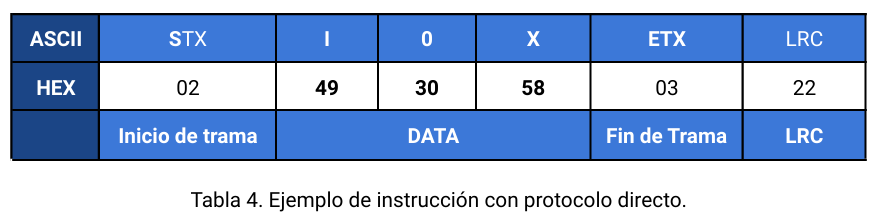
\includegraphics[width=0.9\linewidth]{Img/image4.png}
        \label{fig:placeholder}
    \end{figure}

    {\color{red} \subsubsection*{Leer estado}}

    Para determinar el estado en que se encuentra la impresora fiscal, se envía un Enquirement (ENQ=0x05h)

    Este comando se envía a la impresora fiscal para determinar el estado en que se encuentra y si existe un error, evaluarlo. Cuando se envía un ENQ a la impresora, esta responde con una trama similar a la de recepción, donde DATA es un par de bytes que contienen la información del Estado y el posible Error de la impresora.

    La impresora responderá una trama con la siguiente estructura:

    \begin{figure} [H]
        \centering
        
\includegraphics[width=0.8\linewidth]{Img/image5.png}
        \label{fig:placeholder}
    \end{figure}

    Dónde:

    \begin{itemize}
        \item STS1 corresponde al Estado de la impresora.
        \item STS2 corresponde al Error de la impresora.
    \end{itemize}

    Las siguientes tablas contienen los valores frecuentes para los bytes de Status (STS1) y Error (STS2) de las impresoras fiscales:

    \begin{figure} [H]
        \centering
        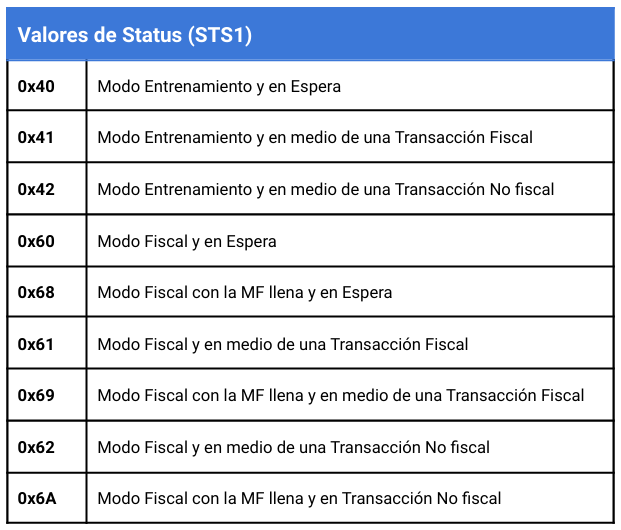
\includegraphics[width=0.7\linewidth]{Img/image6.png}
        \label{fig:placeholder}
    \end{figure}

    \begin{figure} [H]
        \centering
        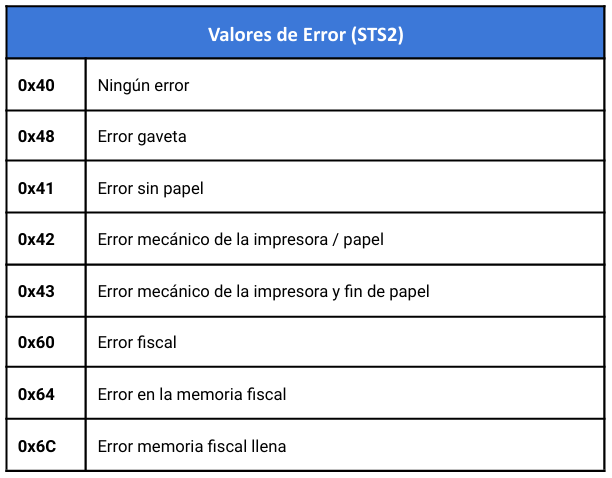
\includegraphics[width=0.7\linewidth]{Img/image7.png}
        \label{fig:placeholder}
    \end{figure}

    {\color{red} \subsubsection*{Leer status de información}}

    Se puede tener acceso a la información que posee la impresora Fiscal, dicha información es repartida en diversos status informativos.

    En el caso de protocolo directo, debe enviar la trama de la solicitus que desee y leer la respuesta en el puerto de comunicaciones basándose en las tablas de respuesta aquí discritas.

    \paragraph{STATUS S1}

    Este comando permite consultar información referente a parámetros de la impresora fiscal como Serial de la misma, RIF, datos de factura, entre otros. Este comando es posible ejecutarlo en cualquier condición.

    \begin{figure} [H]
        \centering
        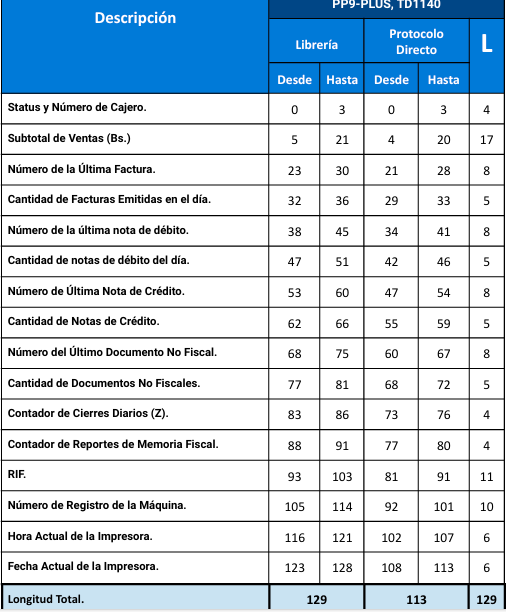
\includegraphics[width=1\linewidth]{Img/image10.png}
        \label{fig:placeholder}
    \end{figure}
    
    
    \subsection*{Dificultades}

    \subsection*{Notas}

    Durante el transcurso de la semana se buscara cumplir con los objetivos de las semanas 3 y 4 del plan de trabajo, que se centran en el \textbf{Diseño de la arquitectura IoT} y el \textbf{Diseño de la arquitectura de comunicaciones MQTT}, se debe definir los planos técnicos y lógicos que permitirán que el ESP32 actúe como el puente entre el equipo fiscal y la nube.

    A continuación, se detalla qué debería abarcar exactamente cada actividad:

    \begin{enumerate}
        \item \textbf{Diseño de la arquitectura IoT:} Esta actividad debe definir la estructura macro del sistema, integrando el hardware, los protocolos y la plataforma de visualización.

        \begin{itemize}
            \item \textbf{Diagrama de bloques del sistema:} Debes representar el flujo de datos desde el equipo fiscal hacia el ESP32 (vía serial RS232), y desde este hacia el servidor MQTT y el dashboard final.
            \item \textbf{Interfaz física (Capa de Dispositivo):} Especificar la conexión serial con la impresora utilizando el estándar RS232 con los parámetros técnicos obligatorios: 9600 bps, 8 bits de datos, Paridad Par y 1 bit de parada.
            \item \textbf{Capa de Red:} Definir el uso de la red Wi-Fi como medio de transporte para los paquetes MQTT.
            \item \textbf{Definición de datos operativos:} Determinar exactamente qué campos del manual (como el Status S1 o S2) se van a recolectar (Serial, RIF, actividad de impresión, errores) para ser transmitidos.
        \end{itemize}

        \item \textbf{Diseño de la arquitectura de comunicaciones MQTT:} Aquí se debe configurar la lógica del protocolo para garantizar una comunicación segura y confiable, aprovechando que el ESP-MQTT ya soporta MQTT v5.0.

        \begin{itemize}
            \item \textbf{Estructura de Tópicos (Topic Tree):} Diseñar una jerarquía de tópicos eficiente y descriptiva (ej. \texttt{empresa/dispositivo01/estado}), evitando el uso de espacios o barras iniciales innecesarias.
            \item \textbf{Niveles de Calidad de Servicio (QoS):} Decidir qué nivel de QoS usarás. Para datos críticos fiscales, se recomienda QoS 1 (al menos una vez) o QoS 2 (exactamente una vez) para evitar pérdida de información.
            \item \textbf{Gestión de Sesiones y Mensajes:}

            \begin{itemize}
                \item \textbf{Sesiones Persistentes:} Definir si el broker debe almacenar mensajes mientras el ESP32 esté offline.
                \item \textbf{Last Will and Testament (LWT):} Configurar un "testamento" para que el servidor notifique automáticamente al dashboard si el equipo fiscal se desconecta de forma inesperada.
            \end{itemize}
            \item \textbf{Seguridad:} Definir los mecanismos de autenticación (usuario y contraseña) y el uso de TLS/SSL para el cifrado de la comunicación con el servidor remoto.
            \item \textbf{Propiedades de MQTT v5.0:} Evaluar el uso de Topic Aliases para reducir el tamaño de los paquetes y User Properties para enviar metadatos adicionales sin afectar el payload.
        \end{itemize}
    \end{enumerate}

    Al finalizar esta semana, se debería contar con diagramas de flujo y una tabla de especificaciones que dicten cómo se programará el firmware y se configurará el servidor en las etapas posteriores del cronograma.

    {\color{red} \subsubsection*{Diagrama de arquitectura IoT}}

    \begin{figure} [H]
        \centering
        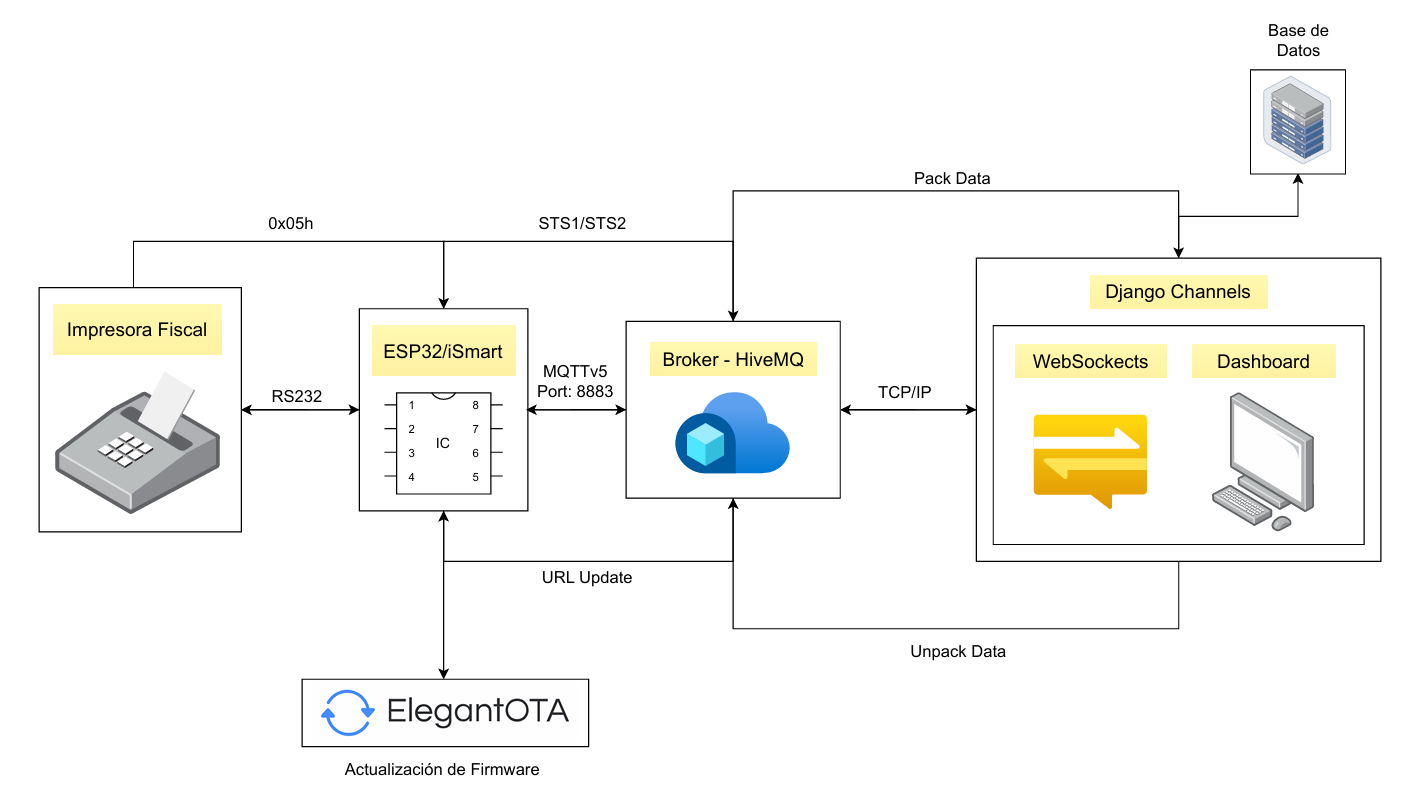
\includegraphics[width=0.9\linewidth]{Img/image8.png}
        \caption{Arquitectura diseñada para el sistema IoT.}
        \label{fig:placeholder}
    \end{figure}

    {\color{red} \subsubsection*{Diagrama de arquitectura de comunicación MQTT}}

    \begin{figure} [H]
        \centering
        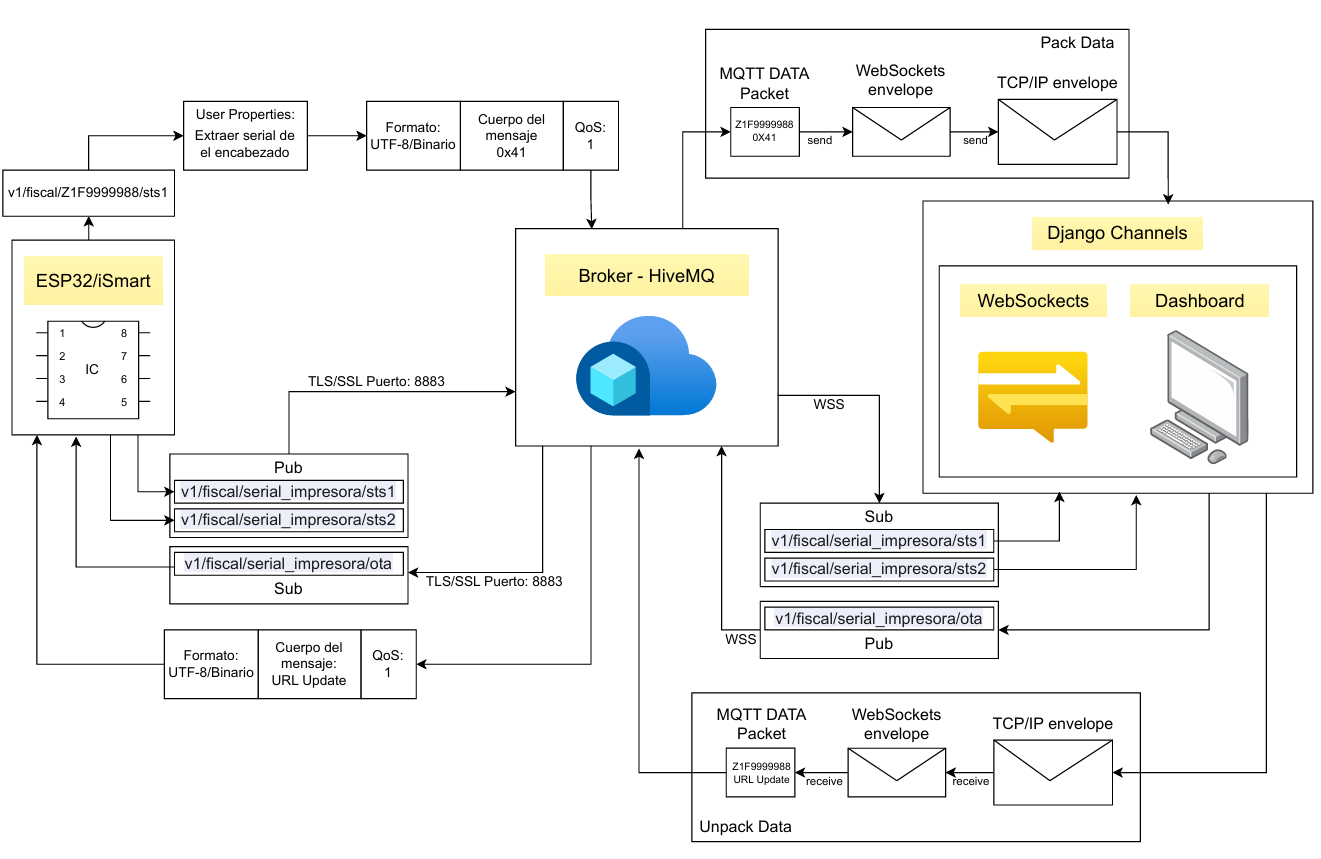
\includegraphics[width=0.9\linewidth]{Img/image9.png}
        \caption{Arquitectura diseñada para la comunicación MQTT.}
        \label{fig:placeholder}
    \end{figure}

    \section*{Fecha: 27/01/2026}

    \subsection*{Actividades}

    \begin{itemize}
        \item Comenzar codigo para leer y procesar los datos en el ESP32
    \end{itemize}

    \subsection*{Aprendizajes}

    {\color{red} \subsubsection*{Conceptos básicos de una Tarea (Task)}}
    
    Una tarea es simplemente una función de C que contiene un bucle infinito (while(1)) y que nunca debe retornar. En nuestro caso, necesitamos al menos una tarea que se encargue de "interrogar" a la impresora periódicamente.
    
    La función principal para crear tareas es:

    \begin{itemize}
        \item \texttt{xTaskCreate()}: Crea una tarea y deja que el sistema decida en qué núcleo ejecutarla.
        \item \texttt{xTaskCreatePinnedToCore()}: Muy recomendada en el ESP32 para asegurar que una tarea (como la de la impresora) no interfiera con las tareas críticas de red (como Wi-Fi/MQTT).
    \end{itemize}
    
    \paragraph{Ejemplo práctico: Tarea de Interrogación (Polling)}
    
    Basado en el flujo de diseño donde el ESP32 debe enviar un \texttt{0x05h} (ENQ) para solicitar el estado, así se vería la estructura de una tarea simple:

    \begin{verbatim}
        // Esta es la función de la tarea
        void printer_polling_task(void *pvParameters) {
            uint8_t enq_cmd = 0x05; // Carácter ENQ según el manual
            
            while(1) {
                // 1. Enviar el comando por UART
                uart_write_bytes(UART_NUM_1, (const char*) &enq_cmd, 1);
                
                // 2. Esperar un tiempo antes de volver a preguntar
                // Es vital usar vTaskDelay para no bloquear el procesador
                vTaskDelay(pdMS_TO_TICKS(5000)); // Pregunta cada 5 segundos
            }
        }
        
        // Así la creas en tu app_main()
        void app_main(void) {
            // ... Configuración de UART que ya hiciste ...
        
            // Crear la tarea: (función, nombre, stack, parámetros, prioridad, handle)
            xTaskCreate(printer_polling_task, "printer_task", 4096, NULL, 5, NULL);
        }
    \end{verbatim}

    Los pines UART en nuestro ESP32 son:
    
    \begin{itemize}
        \item UART0: TX (GPIO1), RX (GPIO3)
        \item UART1: TX (GPIO10), RX (GPIO9). IMPORTANTE: En el DevKitC V4, estos pines suelen estar conectados a la memoria Flash interna. Si se intenta usarlos, el ESP32 se reiniciará constantemente o no encenderá. No usar. Si se necesita usar, se pueden mover el UART1 hacia otros pines libre, por ejemplo: GPIO18 (TX) y GPIO19 (RX).
        \item UART2: TX (GPIO17), RX (GPIO16)
    \end{itemize} 

    \subsection*{Dificultades}

    Para simular una impresora fiscal desde mi computador necesito conectar otro puerto serial (UART2) en mi ESP32.

    \subsection*{Notas}

    Tratando de adaptar un cable RJ12, para comunicar el computador y el ESP32, por instrucción de Antonio aprendi a soldar cables.

    \section*{Fecha: 28/01/2026}

    \subsection*{Actividades}

    \begin{itemize}
        \item Lograr doble puerto serial en el computador
        \item Probar código hecho el día anterior
        \item Seguir avanzando en la version 1 del firmware ESP32
    \end{itemize}

    \subsection*{Aprendizajes}

    Logrando probar el codigo hecho el dia anterior probamos diferentes resultados, desde tramas de bits erroneas

    \begin{figure} [H]
        \centering
        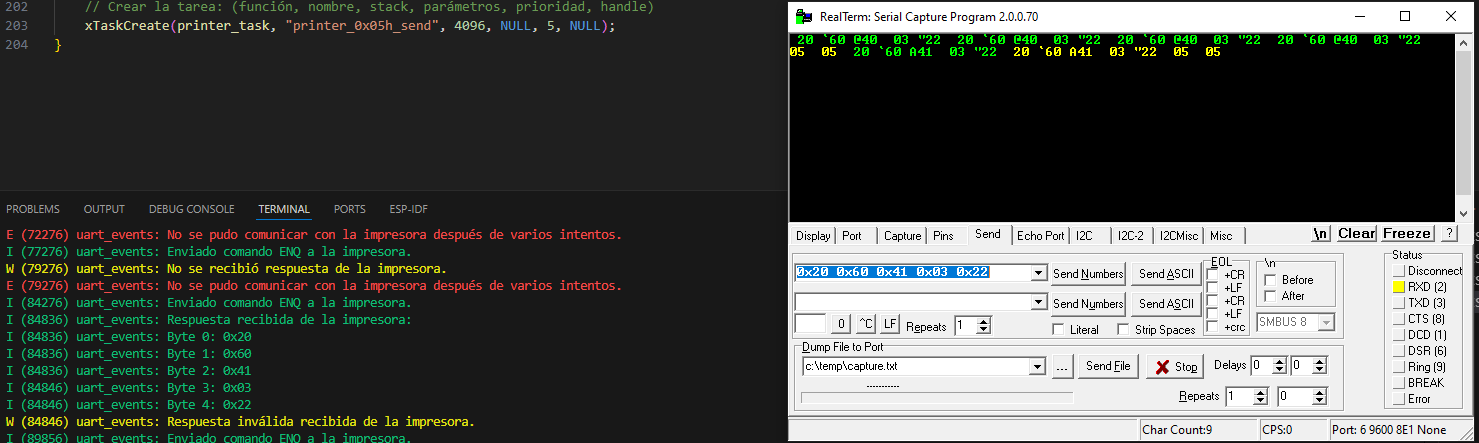
\includegraphics[width=1\linewidth]{Img/image11.png}
        \caption{Respuesta obtenida al enviar la trama: 0x20 0x60 0x41 0x03 0x22.}
        \label{fig:placeholder}
    \end{figure}

    Hasta tramas de bits correctas y publicando el estado de la impresora por puerto serial:

    \begin{figure} [H]
        \centering
        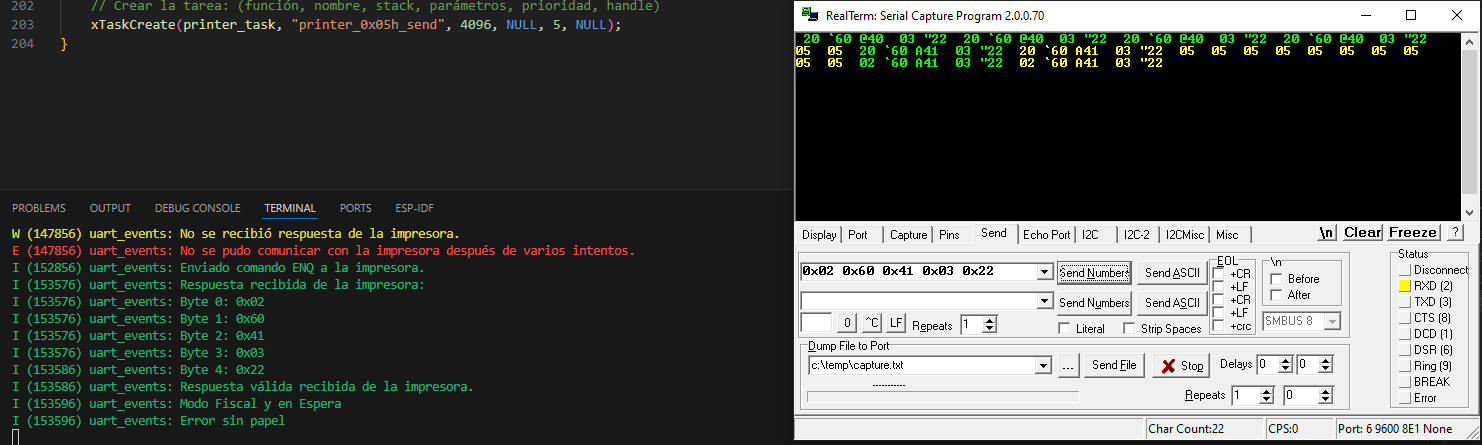
\includegraphics[width=1\linewidth]{Img/image12.png}
        \caption{Respuesta obtenida al enviar la trama: 0x02 0x60 0x41 0x03 0x22.}
        \label{fig:placeholder}
    \end{figure}

    \subsection*{Dificultades}

    Se tuvieron dificultades en el cable prolofic por temas de drivers, pero con instrucción de Elio se pudo solventar.

    En el caso del segundo monitor, Realterm, no es posible enviar la una cadena de bits tan larga como lo es STATUS S1, se barajea la opción de cambiar este monitor si no se resuelve el problema.

    \subsection*{Notas}

    Continuamos el codigo buscando procesar los datos de STATUS S1, donde por precaución se extraeran todos, en un futuro de no necesitarlos se eliminara del código.

    \section*{Fecha: 30/01/2026}

    \subsection*{Actividades}

    \begin{itemize}
        \item Culminar la captura y procesamiento de datos para SATATUS S1
        \item Mejorar eficiencia y robustez del código
    \end{itemize}

    \subsection*{Aprendizajes}

    \subsection*{Dificultades}

    Mandar la trama de datos de la impresora a traves del Realterm se volvio un proceso complicado e ineficiente, ya que este tenia combinaciones de caracteres (hexadecimal y ASCII) por lo que se recurrio al uso de un Scrip en python que automaticamente simulaba el comportamiento de una impresora fiscal, mediante el siguiente codigo:

    \begin{verbatim}
import serial
import time
import sys

def simulador_depuracion():
    """Simulador con depuración detallada"""
    try:
        ser = serial.Serial(
            port='COM6',
            baudrate=9600,
            bytesize=serial.EIGHTBITS,
            parity=serial.PARITY_EVEN,
            stopbits=serial.STOPBITS_ONE,
            timeout=1
        )
        
        print("=" * 60)
        print("SIMULADOR DE IMPRESORA FISCAL - MODO DEPURACIÓN")
        print("=" * 60)
        print(f"Puerto: {ser.port}")
        print(f"Baudrate: {ser.baudrate}")
        print(f"Bytesize: {ser.bytesize}")
        print(f"Parity: {ser.parity}")
        print(f"Stopbits: {ser.stopbits}")
        print("=" * 60)
        print("Esperando comandos...")
        print("Presiona Ctrl+C para salir")
        print("=" * 60)
        
        contador = 0
        
        while True:
            # Leer datos byte por byte
            if ser.in_waiting > 0:
                byte = ser.read(1)
                contador += 1
                
                print(f"\n[{contador}] Byte recibido:")
                print(f"  Hexadecimal: 0x{byte.hex().upper()}")
                print(f"  Decimal: {int.from_bytes(byte, 'big')}")
                print(f"  Binario: {bin(int.from_bytes(byte, 'big'))[2:].zfill(8)}")
                
                # Intentar interpretar como ASCII
                try:
                    ascii_char = byte.decode('ascii')
                    print(f"  ASCII: '{ascii_char}'")
                except:
                    print(f"  ASCII: No es ASCII válido")
                
                # Mostrar tipo de comando
                if byte == b'\x05':
                    print(f"  TIPO: ENQ (Consulta de estado)")
                elif byte == b'\x4C':
                    print(f"  TIPO: STATUS S1")
                elif byte == b'\x02':
                    print(f"  TIPO: STX (Inicio de trama)")
                elif byte == b'\x03':
                    print(f"  TIPO: ETX (Fin de trama)")
                elif byte == b'\x15':
                    print(f"  TIPO: NAK (No reconocimiento)")
                elif byte == b'\x06':
                    print(f"  TIPO: ACK (Reconocimiento)")
                else:
                    print(f"  TIPO: Desconocido")
                
                # Responder según el byte recibido
                if byte == b'\x05':  # ENQ
                    print("  -> Enviando respuesta ENQ: 0x02 0x60 0x40 0x03")
                    respuesta = b'\x02\x60\x40\x03'
                    ser.write(respuesta)
                    ser.flush()
                    
                elif byte == b'\x4C':  # STATUS S1
                    print("  -> Enviando respuesta STATUS S1")
                    # Construir datos de prueba
                    datos = "00100000000000000000000000000000000000000000
                    0000000000000000000000000000000000000J3121711970
                    Z1F9999988123000300126"
                    
                    # Enviar STX + datos + ETX
                    respuesta = b'\x02' + datos.encode('ascii') + b'\x03'
                    print(f"  -> Longitud respuesta: {len(respuesta)} bytes")
                    print(f"  -> STX: 0x02, ETX: 0x03")
                    print(f"  -> Datos ASCII: {len(datos)} caracteres")
                    
                    ser.write(respuesta)
                    ser.flush()
                    
                else:
                    print(f"  -> Byte desconocido, NO respondiendo")
                    # NO enviar NAK para evitar el bucle infinito
                    # ser.write(b'\x15')
                
                print("-" * 40)
            
            time.sleep(0.01)
            
    except KeyboardInterrupt:
        print("\n\nSimulador detenido por usuario")
    except Exception as e:
        print(f"\nError: {e}")
    finally:
        if 'ser' in locals() and ser.is_open:
            ser.close()
            print("Puerto serial cerrado")

if __name__ == "__main__":
    simulador_depuracion()
    \end{verbatim}

    \subsection*{Notas}

    Se logró mandar e interpretar el comando STATUS S1 en nuestra primera versión de firmware para ESP32 obteniendo este primer resultado preliminar que luego mandaremos a traves de protocolo MQTT:

    \newpage

    \begin{verbatim}
        I (13297) uart_events: === STATUS S1 ===
        I (13297) uart_events: Número de Cajero: [0010]
        I (13307) uart_events: Subtotal Ventas: [00000000000000000]
        I (13307) uart_events: Última Factura: [00000000]
        I (13317) uart_events: Facturas hoy: [00000]
        I (13317) uart_events: RIF: [J3121711970]
        I (13317) uart_events: Número Registro: [Z1F9999988]
        I (13317) uart_events: RIF: [J3121711970]
        I (13317) uart_events: Número Registro: [Z1F9999988]
        I (13317) uart_events: Número Registro: [Z1F9999988]
        I (13327) uart_events: Hora: [123000]
        I (13327) uart_events: Fecha: [300126]
    \end{verbatim}  

    Es evidente que hay redundancias y repeticiones, por lo cual se trabajara en solventar, pero tambien vemos que la data esta organizada correctamente y los datos coinciden con sus respectivos campos.

    Se logró conseguir una version final que funciona correctamente:

    \begin{verbatim}
I (12278) uart_events: Enviado comando ENQ a la impresora.
I (12298) uart_events: Respuesta válida recibida de la impresora.
I (12298) uart_events: Modo Fiscal y en Espera
I (12298) uart_events: Ningún error
I (12398) uart_events: Enviado carácter STATUS S1 (0x4C) a la impresora.
I (17898) uart_events: Procesando STATUS S1, len=116
I (17898) uart_events: STX encontrado en posición: 0
I (17898) uart_events: === STATUS S1 ===
I (17898) uart_events: Número de Cajero: [0010]
I (17898) uart_events: Subtotal Ventas: [00000000000000000]
I (17908) uart_events: Número de Última Factura: [00000000]
I (17908) uart_events: Cantidad de Facturas Emitidas: [00000]
I (17918) uart_events: Número de Última Nota de Débito: [00000000]
I (17918) uart_events: Cantidad de Notas de Débito del Día: [00000]
I (17928) uart_events: Número de Última Nota de Crédito: [00000000]
I (17938) uart_events: Cantidad de Notas de Crédito: [00000]
I (17938) uart_events: Número del Último Documento No Fiscal: [00000000]
I (17948) uart_events: Cantidad de Documentos No Fiscales: [00000]
I (17948) uart_events: Contador de Cierres Diarios (Z): [0000]
I (17958) uart_events: Contador de Reportes de Memoria Fiscal: [0000]
I (17968) uart_events: RIF: [J3121711970]
I (17968) uart_events: Número Registro de la Máquina: [Z1F9999988]
I (17978) uart_events: Hora Actual de la Impresora: [123000]
I (17978) uart_events: Fecha Actual de la Impresora: [300126]
    \end{verbatim}

    Falto por mejorar la eficiencia y robustez del codigo, una vez logrado eso se avanzará con la siguiente fase del proyecto "Implementación de comunicación Wi-Fi y MQTT en el ESP32"

    \section*{Fecha: 02/02/2026}

    \subsection*{Actividades}

    \begin{itemize}
        \item Parametrizar variables de información que se enviaran a través de MQTT
        \item Mejorar eficiencia de código firmware V1
        \item (OPCIONAL) Comenzar adaptación a WiFi y MQTT, comenzando Firmware V2
    \end{itemize}

    \subsection*{Aprendizajes}

    Mejorando la estructura del codigo, buscaré implementar las siguientes mejoras:

    \begin{itemize}
        \item Sistema de reconexión y timeouts.
        \item Seguridad en acceso de memoria.
        \item Configuración centralizada (archivo header).
        \item Mejorar manejo de errores.
        \item Optimización del performance, volviendolo mas personalizado hacia su objetivo.
    \end{itemize}

    Se implementó la función \texttt{xTaskGetTickCount()} donde devuelve el conteo total de "ticks" (ciclos de reloj del sistema) que han transcurrido desde que el planificador de tareas (scheduler) se inició tras el arranque del ESP32. Esta función es vital para cumplir con los objetivos de "mecanismos de diagnóstico, reconexión y trazabilidad" definidos en el plan de pasantía.    

    \subsection*{Dificultades}

    Implementando una nueva versión que sea escalable entramos en la problematica de "demasiado uso de memoria":

    \begin{figure} [H]
        \centering
        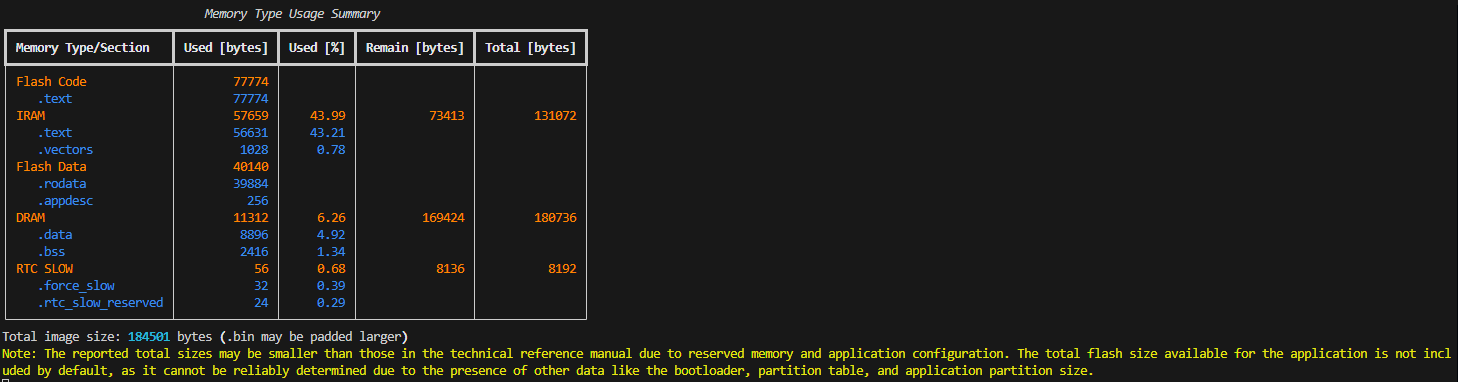
\includegraphics[width=1\linewidth]{Img/image13.png}
        \caption{Uso excesivo de memoria IRAM (43.99\%).}
        \label{fig:placeholder}
    \end{figure}

    Siendo esta la implementación de una unica tarea, por lo tanto se toma como una actualización pero se buscara realizar una version optimizada de la misma.

    \subsection*{Notas}

    Vemos un vistazo de como serán los tópicos enviados a través de MQTT, culminando una primera versión para la captura y procesamiento de datos:

    \begin{figure} [H]
        \centering
        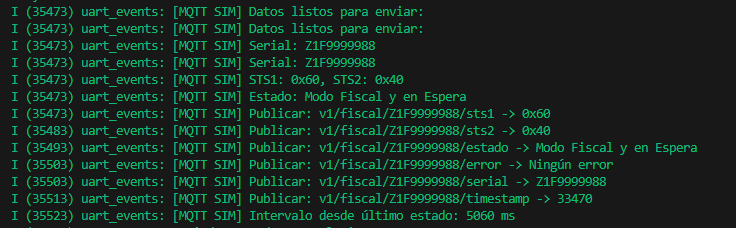
\includegraphics[width=0.9\linewidth]{Img/image14.png}
        \caption{Tópicos para protocolo MQTT y datos contenidos en el tópico.}
        \label{fig:placeholder}
    \end{figure}

    Con estos datos ya parametrizados, el código esta casi listo para comenzar la implementación WiFi y MQTT, no obstante, en estos momentos centrare el trabajo en resolver la alta demanda de memoria que actualmente tiene el código. Una vez resuelto, si avanzaremos con la implementación WiFi y MQTT.

    \section*{Fecha: 03/02/2026}

    \subsection*{Actividades}

    \begin{itemize}
        \item Realizar conexión WiFi para Firmware V1.
        \item Realizar conexión MQTT para Firmware V1.
        \item Visualizar primeros datos a través de broker HiveMQ en la nube.
    \end{itemize}

    \subsection*{Aprendizajes}

    Usando programación modular para gestionar las extensas tareas del firmware, se propone la siguiente estructura:

    \begin{figure} [H]
        \centering
        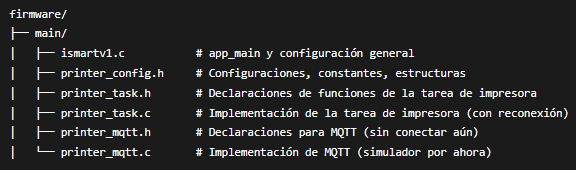
\includegraphics[width=0.9\linewidth]{Img/image15.png}
        \caption{Estructura modular para Firmware V1.}
        \label{fig:placeholder}
    \end{figure}

    Dicha estructura mostro un aumento de 0.11\% en el uso de la memoria IRAM, pero en investigaciones pude encontrar que, un uso del 44.01\% de la IRAM (Instruction RAM) en un proyecto basado en el ESP32 utilizando el framework ESP-IDF no se considera excesivo, pero sí es un valor que requiere atención y monitoreo constante a medida que se integren más funcionalidades.

    \begin{figure} [H]
        \centering
        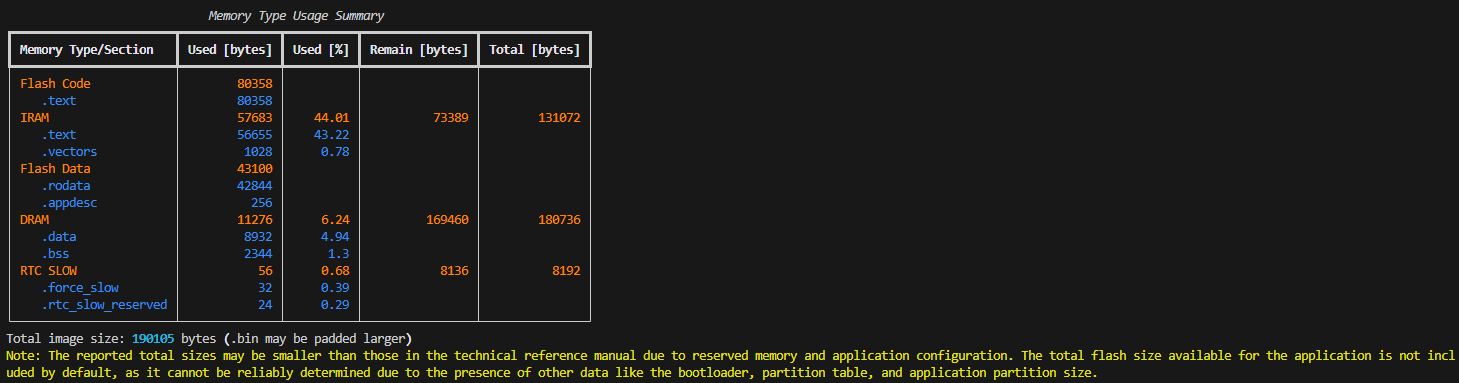
\includegraphics[width=0.9\linewidth]{Img/image16.png}
        \caption{Tabla del uso de memoria para programación modular.}
        \label{fig:placeholder}
    \end{figure}

    Se adjuntan ejemplos de uso:

    \begin{figure} [H]
        \centering
        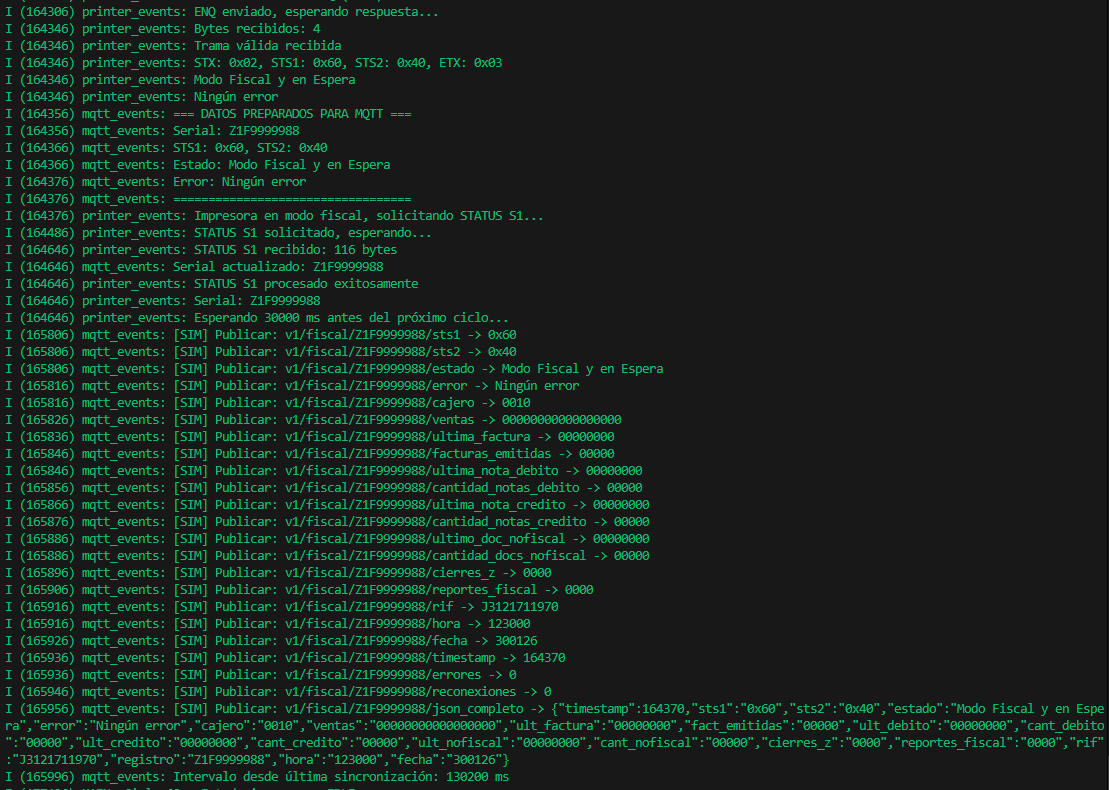
\includegraphics[width=0.9\linewidth]{Img/image17.png}
        \caption{Muestra de procesamiento de datos capturados y preparados para enviar por MQTT.}
        \label{fig:placeholder}
    \end{figure}

    \begin{figure} [H]
        \centering
        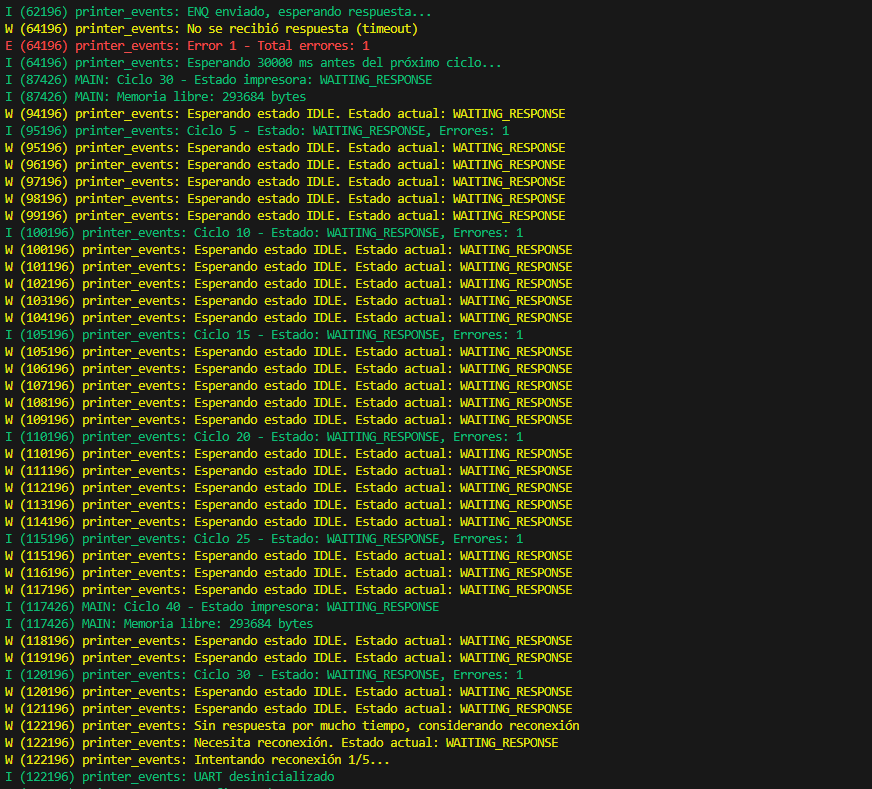
\includegraphics[width=0.9\linewidth]{Img/image18.png}
        \caption{Muestra de funcionalidad de reconexión.}
        \label{fig:placeholder}
    \end{figure}

    \subsection*{Dificultades}

    \subsection*{Notas}

    Ahora avanzaremos a la siguiente fase del proyecto "Implementación de comunicación Wi-Fi y MQTT en el ESP32" para ello se implementará una adaptación del mini-proyecto realizado en semana 1, a lo que tenemos de simulador MQTT en la versión actual.

    \begin{figure} [H]
        \centering
        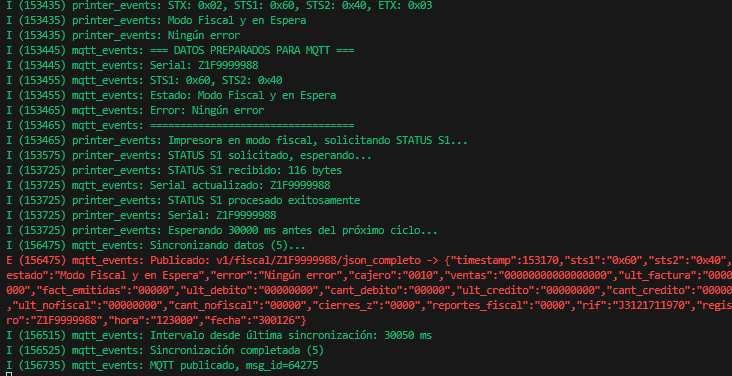
\includegraphics[width=0.9\linewidth]{Img/image19.png}
        \caption{Prueba de funcionamiento para datos enviados desde MQTT.}
        \label{fig:placeholder}
    \end{figure}

    \begin{figure} [H]
        \centering
        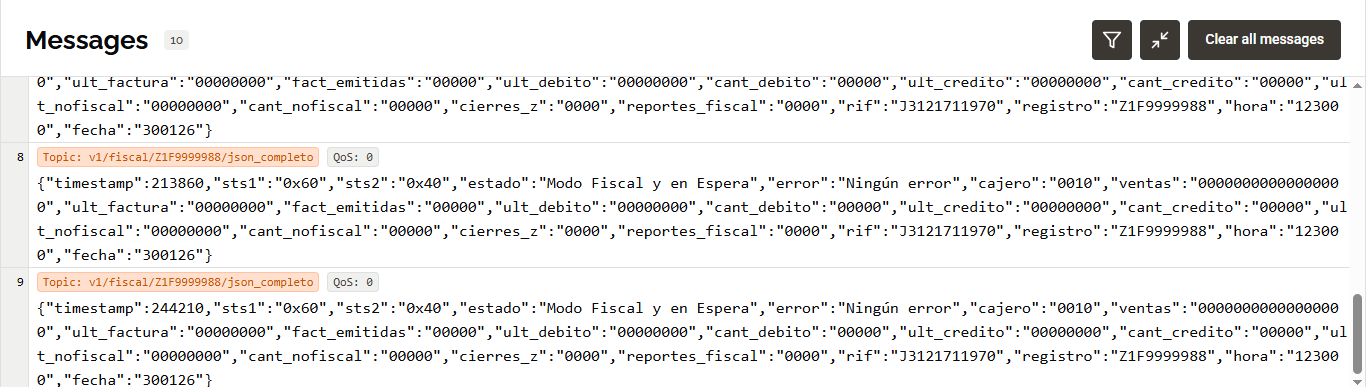
\includegraphics[width=0.9\linewidth]{Img/image20.png}
        \caption{Visualización de datos a través de broker HiveMQ.}
        \label{fig:placeholder}
    \end{figure}

    Se logró enviar los datos a través de MQTT hacia el broker escogido. Además se implemento un sistema de reconexión en caso de si se va el wifi o se pierde conexion con la impresora. Se concluye que los objetivos del dia fueron cumplidos.

    \section*{Fecha: 04/02/2026}

    \subsection*{Actividades}

    \begin{itemize}
        \item Crear casos para estados \(\neq\) 0x60 donde no se envien todos los datos (esto por que en una impresora real ocurre así).
        \item Implementar LCR del protocolo ENQ y STATUS S1.
        \item Arreglar definiciones redundantes en el codigo.
        \item Mejorar el manejo de IRAM para futuras actualizaciones (seguridad TLS y OTA).
    \end{itemize}

    \subsection*{Aprendizajes}

    \subsection*{Dificultades}

    No se reportan muchos avances, ya que se sigue trabajando en la nueva adaptación que trabaje lo mas fiel posible al protocolo de comunicación de una impresora fiscal.

    \subsection*{Notas}

    Aplique mejoras al simulador (\texttt{impresora.py}) coon el fin de que sea lo mas cercano a una impresora fiscal, y el código de firmware sea lo mas fiel a futuras integraciones fisicas reales. Ahora nuestro simulador maneja LCR, asi como tambien el envio de ACK y NAK.

    \section*{Fecha: 06/02/2026}

    \subsection*{Actividades}

    \begin{itemize}
        \item Corregir incovenientes con el código.
    \end{itemize}

    \subsection*{Aprendizajes}

    {\color{red} \subsubsection*{¿Qué es un Mutex?}}
    
    Imagina que \texttt{mqtt\_data} es un cuaderno donde escribes información.

    \begin{itemize}
        \item La \textbf{Tarea de la Impresora} es alguien que escribe en el cuaderno.

        \item La \textbf{Tarea de MQTT} es alguien que lee del cuaderno para enviar la información a internet.
    \end{itemize}
    
    Si ambos intentan usar el cuaderno al mismo tiempo, uno podría estar leyendo mientras el otro apenas va por la mitad de la escritura, y los datos se enviarían incompletos o corruptos.

    Un Mutex (abreviatura de Mutual Exclusion) es como una llave.

    \begin{itemize}
        \item Para tocar el cuaderno, tienes que pedir la llave.

        \item Si la tienes tú, nadie más puede tocarlo.

        \item Cuando terminas, devuelves la llave para que otro la use.
    \end{itemize}

    \subsection*{Dificultades}

    \begin{figure} [H]
        \centering
        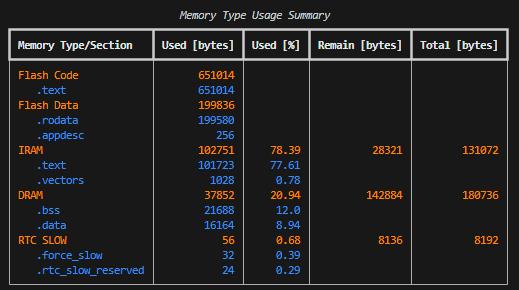
\includegraphics[width=0.9\linewidth]{Img/image21.png}
        \caption{Uso de IRAM con implementación completa muy elevado (78.39\%).}
        \label{fig:placeholder}
    \end{figure}

    \subsection*{Notas}

    Se lograron significativos avances en la mejora de IRAM para la tarea '\texttt{printer\_task.c}' y se buscará seguir avanzando con la misma metodologia con las demas tareas.

    \section*{Fecha: 09/02/2026}

    \subsection*{Actividades}

    \begin{itemize}
        \item Mejorar implementación para \texttt{mqtt\_task.c}
    \end{itemize}

    \subsection*{Aprendizajes}

    Configurando \texttt{menuconfig} logramos una mejora con el uso de la IRAM desactivando la optimizacion por IRAM de la conexion WiFi.

    \begin{figure} [H]
        \centering
        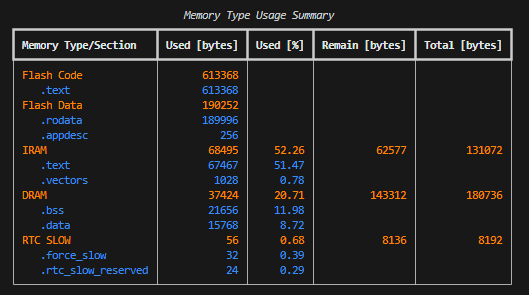
\includegraphics[width=0.9\linewidth]{Img/image22.png}
        \caption{Reducción del uso de la IRAM en un -26.13\% (ahora 52.26\%).}
        \label{fig:placeholder}
    \end{figure}

    \subsection*{Dificultades}

    Con la implementación de ACK y NAK el UART genera mucha basura y no se logra una buena comunicación entre el simulador de impresora y el ESP32, se trabaja para solucionarlo.

    \subsection*{Notas}

    \section*{Fecha: 10/02/2026}

    \subsection*{Actividades}

    \begin{itemize}
        \item Solucionar problemas con la comunicación UART.
    \end{itemize}

    \subsection*{Aprendizajes}
    
    A veces, cuando el edificio se está cayendo, lo mejor es salir, construir una pequeña cabaña al lado y verificar que los cimientos funcionan. Por ello se buscara hacer una prueba del funcionamiento para UART0 y UART1, realizando un proyecto pequeño donde se comuniquen entre si, buscando recepción y transmision optima, libre de ruido y completamente funcional. 

    {\color{red} \subsubsection*{User Properties de MQTTv5}}

    Las User Properties son, básicamente, metadatos en formato clave-valor (UTF-8) que se puede añadir a las cabeceras de casi cualquier paquete MQTT (CONNECT, PUBLISH, SUBSCRIBE, etc.). Las User Properties son como etiquetas adhesivas que pegas por fuera de la caja. Se pueden leer sin abrir el paquete. Esto nos sirve para la implementación web donde no será necesario ver el contenido del mensaje MQTT para direccionarlo a través del backend.

    \subsection*{Dificultades}

    A pesar de haber aplicado un proyecto minimo (y este haya funcionado) nuestro código sigue sin poner leer el estado enviado desde nuestro simulador:

    \begin{figure} [H]
        \centering
        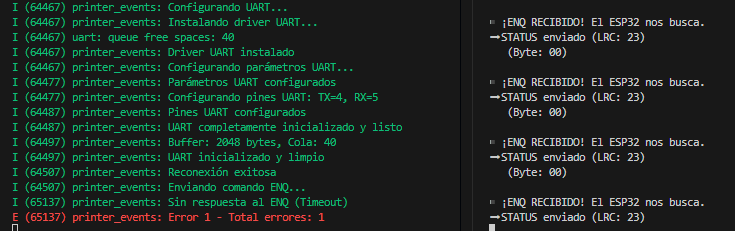
\includegraphics[width=0.9\linewidth]{Img/image23.png}
        \caption{ESP32 no lee STATUS enviado por simulador.}
        \label{fig:placeholder}
    \end{figure}

    \subsection*{Notas}

    Con los problemas solucionados se logro una sincronizacion y optimizacion casi perfectas de esta primera versión de firmware enviando alrededor de mas de 160 mensaje a través de protocolo MQTT sin gran complicación para el firmware.

    \begin{figure} [H]
        \centering
        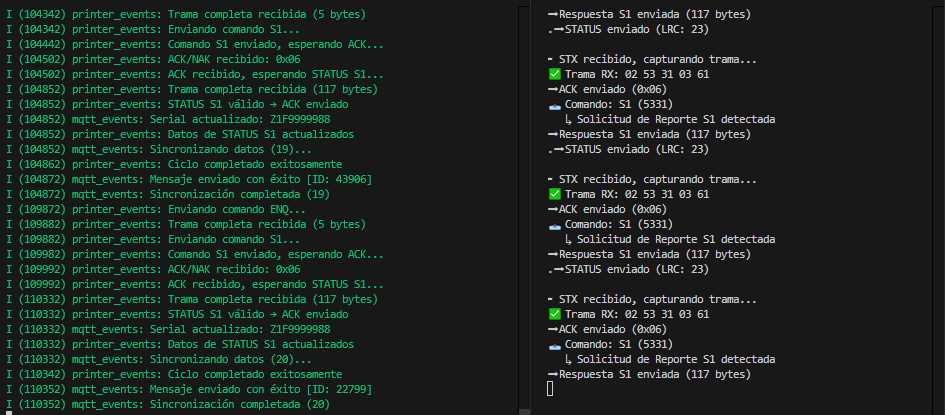
\includegraphics[width=0.9\linewidth]{Img/image24.png}
        \caption{Firmware funcionando correctamente con protocolo MQTT.}
        \label{fig:placeholder}
    \end{figure}

    \section*{Fecha: 11/02/2026}

    \subsection*{Actividades}

    \begin{itemize}
        \item Implementar USER PROPERTIES.
        \item Idear protocolo para username y password.
    \end{itemize}

    \subsection*{Aprendizajes}

    Para las USER PROPERTIES se aplicarón las siguientes declaraciones:

    \begin{verbatim}
        esp_mqtt5_user_property_item_t user_prop_items[] = {
            {"modelo_dispositivo", "HKA80"},
            {"firmware_version", "V1.0"},
            {"serial", mqtt_data.register_number},
            {"tipo_dato", "status_s1"}
        };
    \end{verbatim}

    {\color{red} \subsubsection*{WebSockets: El lenguaje del Dashboard (Servidor a Navegador)}}
    
    Los WebSockets son un protocolo de comunicación bidireccional que permite que el servidor envíe información al navegador de forma instantánea sin que el usuario tenga que refrescar la página. Los WebSockets: actúan como el "cable" siempre conectado entre el servidor y la pantalla del usuario.

    {\color{red} \subsubsection*{Django Channels: El puente (La lógica del Servidor)}}
    
    Django por sí solo está diseñado para responder a peticiones HTTP estándar (el usuario pide una página, el servidor la entrega y se corta la conexión). No sabe "hablar" WebSockets de forma nativa. Aqui es cuando usamos Django Channels, que es una extensión la cual transforma a Django para que pueda manejar protocolos de larga duración como los WebSockets. Actúa como el intermediario que "escucha" los mensajes de MQTT que llegan al broker y los reenvía automáticamente a través de un canal de WebSocket hacia el Dashboard.

     Lo que se propone para nuestra de arquitectura es un flujo de datos:

     \begin{equation}
         \text{TRAMO 1: } \text{ESP32 }  \xrightarrow{MQTT}  \text{Broker}
     \end{equation}

     \begin{equation}
         \text{TRAMO 2: } \text{Servidor (Django Channels) }  \xrightarrow{WebSockets}  \text{Dashboard}
     \end{equation}

     {\color{red} \subsubsection*{Primer proyecto Django}}

     Se comenzó un nuevo mini-proyecto django, con el fin de entrar en contexto con la plataforma.

     \begin{figure} [H]
         \centering
         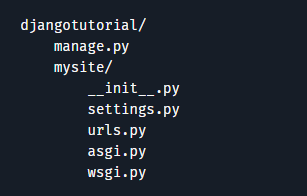
\includegraphics[width=0.6\linewidth]{Img/image25.png}
         \caption{Composición para nuestro primer proyecto en Django.}
         \label{fig:placeholder}
     \end{figure}

     Estos archivos son:

     \begin{itemize}
        \item \texttt{manage.py}: Una utilidad de línea de comandos que te permite interactuar con este proyecto de Django de diversas maneras.
    
        \item \texttt{mysite/}: Un directorio que contiene el paquete de Python de tu proyecto. Su nombre es el nombre del paquete de Python que necesitarás para importar cualquier cosa dentro de él (por ejemplo, \texttt{mysite.urls}).
    
        \item \texttt{mysite/\_\_init\_\_.py}: Un archivo vacío que indica a Python que este directorio debe considerarse un paquete.
    
        \item \texttt{mysite/settings.py}: Configuración de este proyecto de Django. La configuración de Django te explicará todo sobre su funcionamiento.
    
        \item \texttt{mysite/URL.py}: Las declaraciones de URL para este proyecto de Django; una tabla de contenido de su sitio web con Django.
    
        \item \texttt{mysite/asgi.py}: Un punto de entrada para servidores web compatibles con ASGI que atiendan su proyecto.
    
        \item \texttt{mysite/wsgi.py} Un punto de entrada para servidores web compatibles con WSGI que sirvan a su proyecto.
     \end{itemize}

    \subsection*{Dificultades}

    \subsection*{Notas}

    Una vez logrado el firmware para el ESP32, se avanza a la siguiente fase del proyecto, que es implementación de almacenamiento y gestión de datos y desarrollo de la plataforma de visualización.

    \section*{Fecha: 13/02/2026 (Viernes antes de carnaval)} 

    \subsection*{Actividades}

    \begin{itemize}
        \item Culminar prueba inicial de Django Channels.
        \item Jerarquerizar funcionalidades de pagina web y comenzar con lo básico.
    \end{itemize}

    \subsection*{Aprendizajes}

    Mediante django nos conectamos a nuestro broker HiveMQ Cloud y nos traemos los datos de la impresora fiscal para verlos en pantalla, siendo esta una prueba simple de como si es posible comunicar los datos MQTT a la página web.

    \begin{figure} [H]
        \centering
        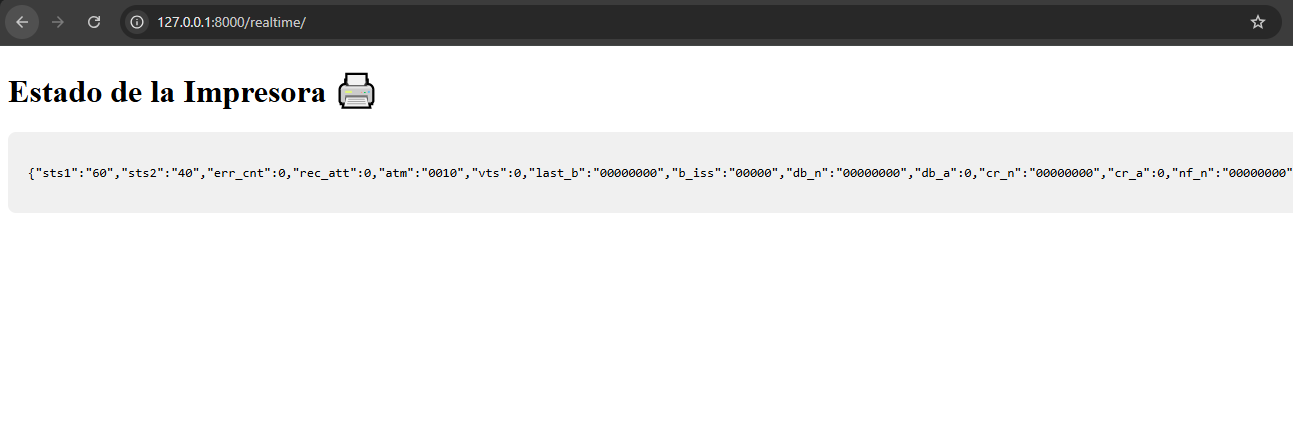
\includegraphics[width=0.9\linewidth]{Img/image27.png}
        \caption{Pueba sencilla de datos MQTT en la web.}
        \label{fig:placeholder}
    \end{figure}

    \subsection*{Dificultades}

    Usar Django Channels requeria la implementación de un servidor de WebSockets, que derivaba a un arduo trabajo de configuración y volveria el proceso mas complicado de llegar, asi que se opto por eliminar esta implementación por completo. No obstante, como HiveMQ Cloud cuenta con conexión WebSocket, fue sencillo conectar la web mediante este puerto 8884, sin necesidad del uso de django channels.

    \subsection*{Notas}

    \section*{Fecha: 18/02/2026 (Miercoles despues de carnaval)}

    \subsection*{Actividades}

    \begin{itemize}
        \item Hacer sistema de registro para interfaz web
        \item Iniciar sección de Device Mgmt despues de registro
    \end{itemize}

    \subsection*{Aprendizajes}

    Comenzando con el desarrollo de la interfaz web, se creo el inicio de esta interfaz con un menu de inicio de sesión:

    \begin{figure} [H]
        \centering
        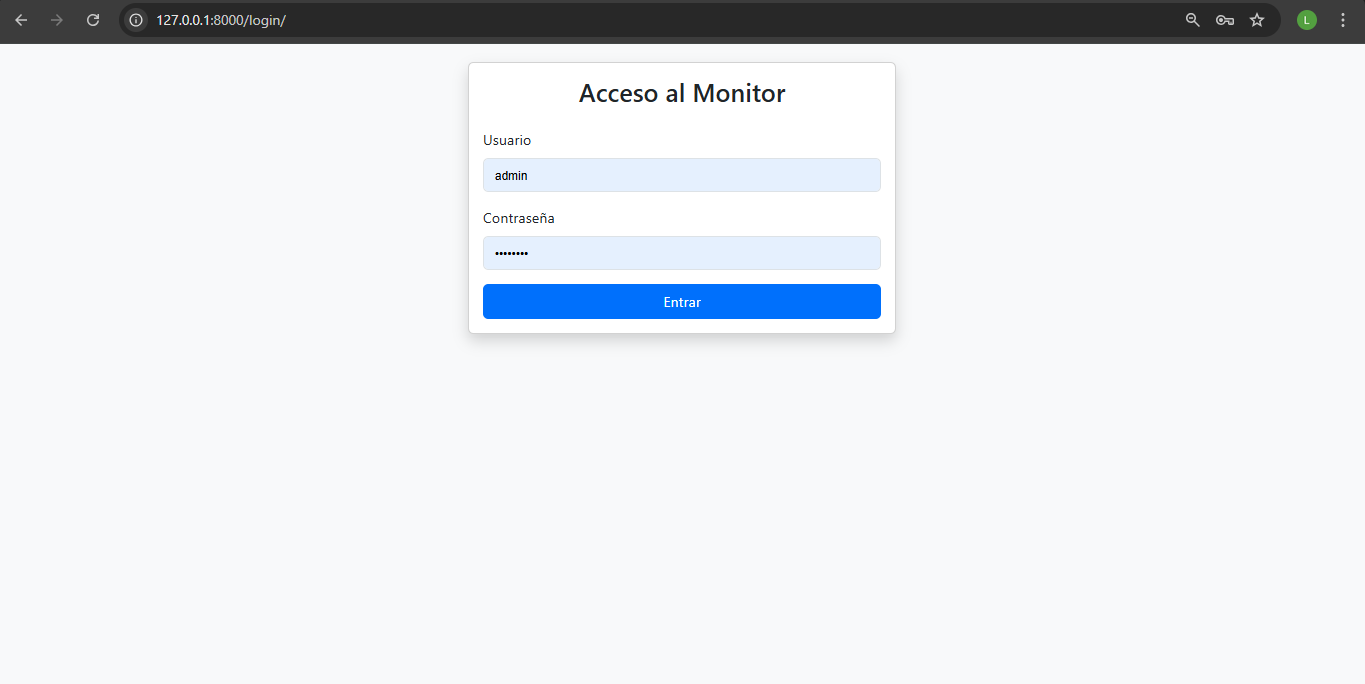
\includegraphics[width=0.9\linewidth]{Img/image28.png}
        \caption{Muestra para la interfaz de inicio de sesión.}
        \label{fig:placeholder}
    \end{figure}

    Y se continuo con el desarrollo del dashboard (interfaz despues del inicio de sesión), donde se podrá vizualizar un resumen de todos los dispositivos en linea y de todos los menú disponibles:

    \begin{figure} [H]
        \centering
        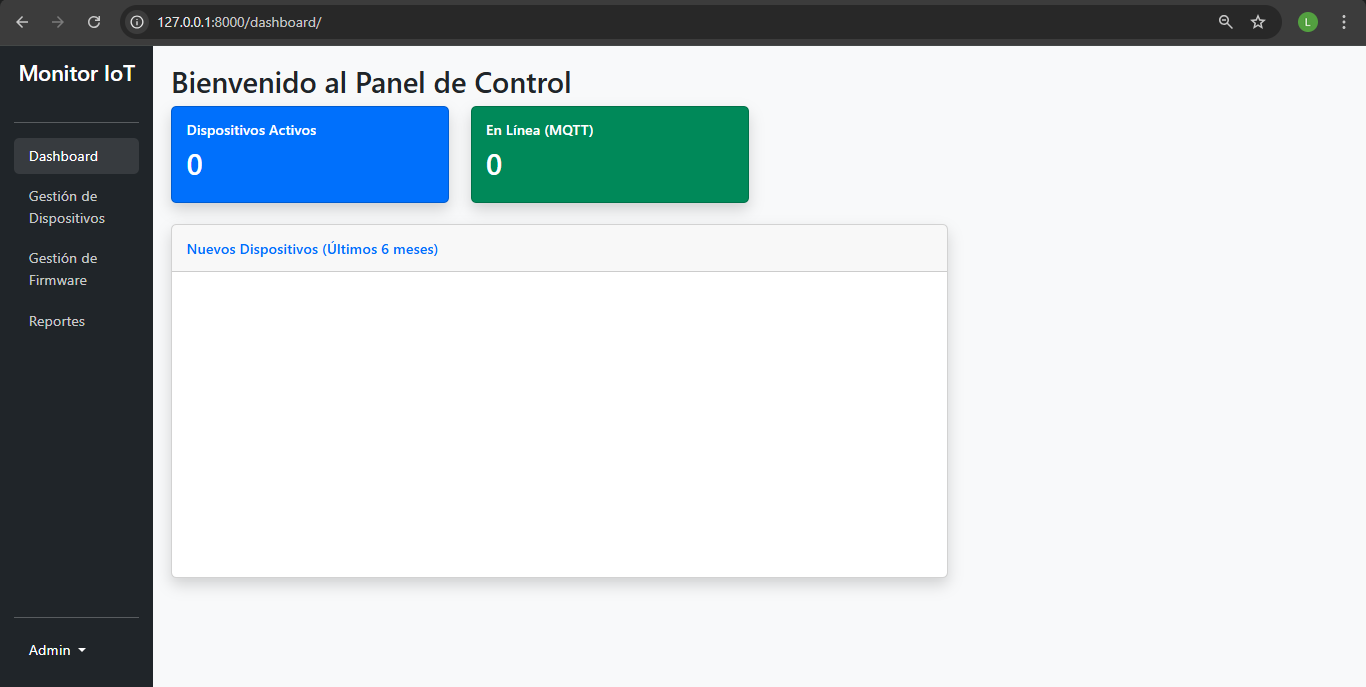
\includegraphics[width=0.9\linewidth]{Img/image29.png}
        \caption{Muestra para el dashboard principal.}
        \label{fig:placeholder}
    \end{figure}

    Avanzando con el proyecto, continuamos con el desarrollo de la gestión de dispositivos, realizando en un primer paso el desarrollo de la interfaz para dicho apartado, donde podemos añadir nuevos dispositivos e incluso cuenta con un buscador para conseguir dispositivos mediante su numero serial o modelo:

    \begin{figure} [H]
        \centering
        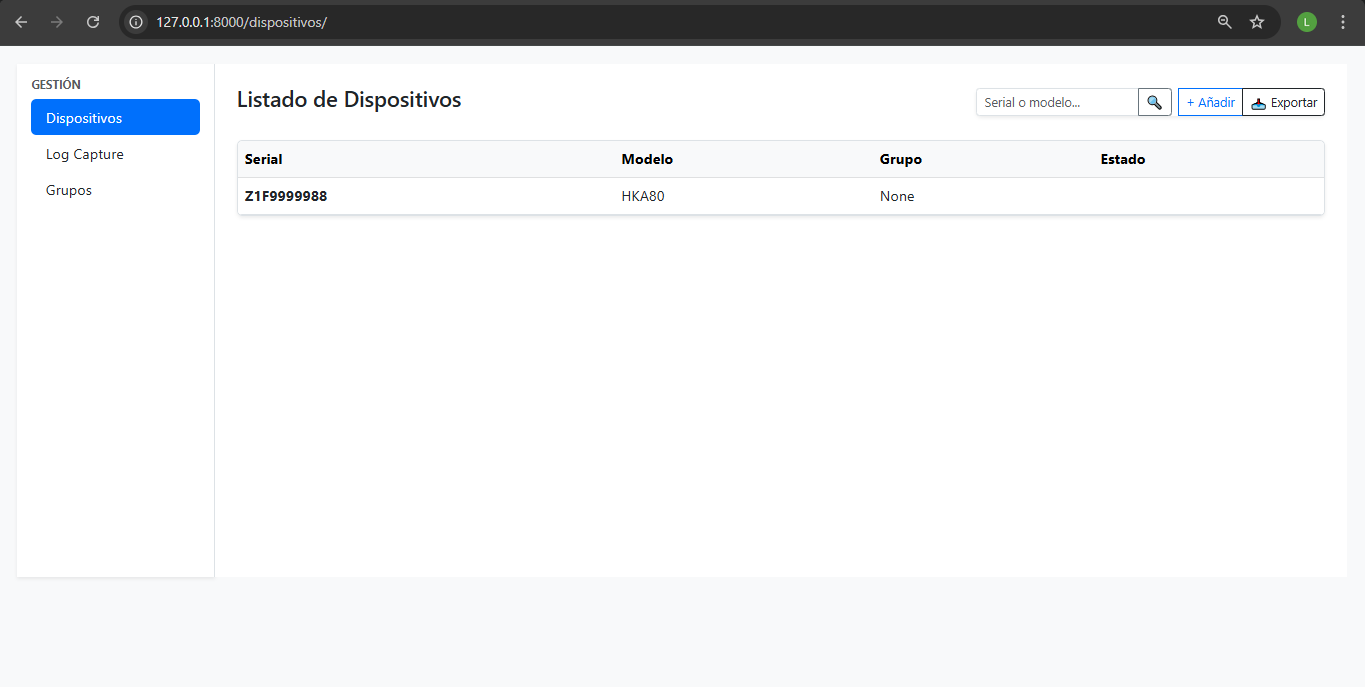
\includegraphics[width=0.9\linewidth]{Img/image30.png}
        \caption{Muestra de la interfaz para Gestión de Dispositivos.}
        \label{fig:placeholder}
    \end{figure}

    En dicha interfaz se desarrollo lo que es la adición de dispositivos:

    \begin{figure} [H]
        \centering
        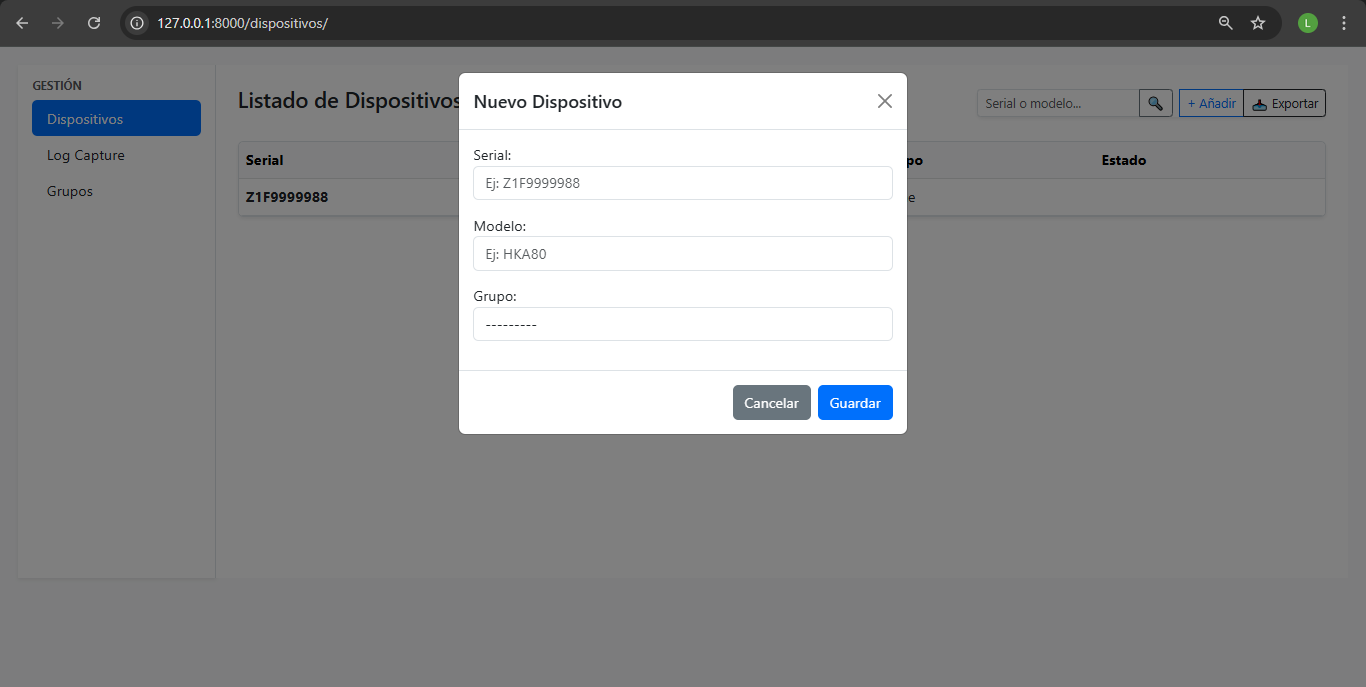
\includegraphics[width=0.9\linewidth]{image31.png}
        \caption{Muestra de interfaz al dale "+ Añadir" en la interfaz "Dispositivo".}
        \label{fig:placeholder}
    \end{figure}

    Una vez registrado el dispositivo podemos visualizar su información (aquí es donde llegan los datos MQTT):

    \begin{figure} [H]
        \centering
        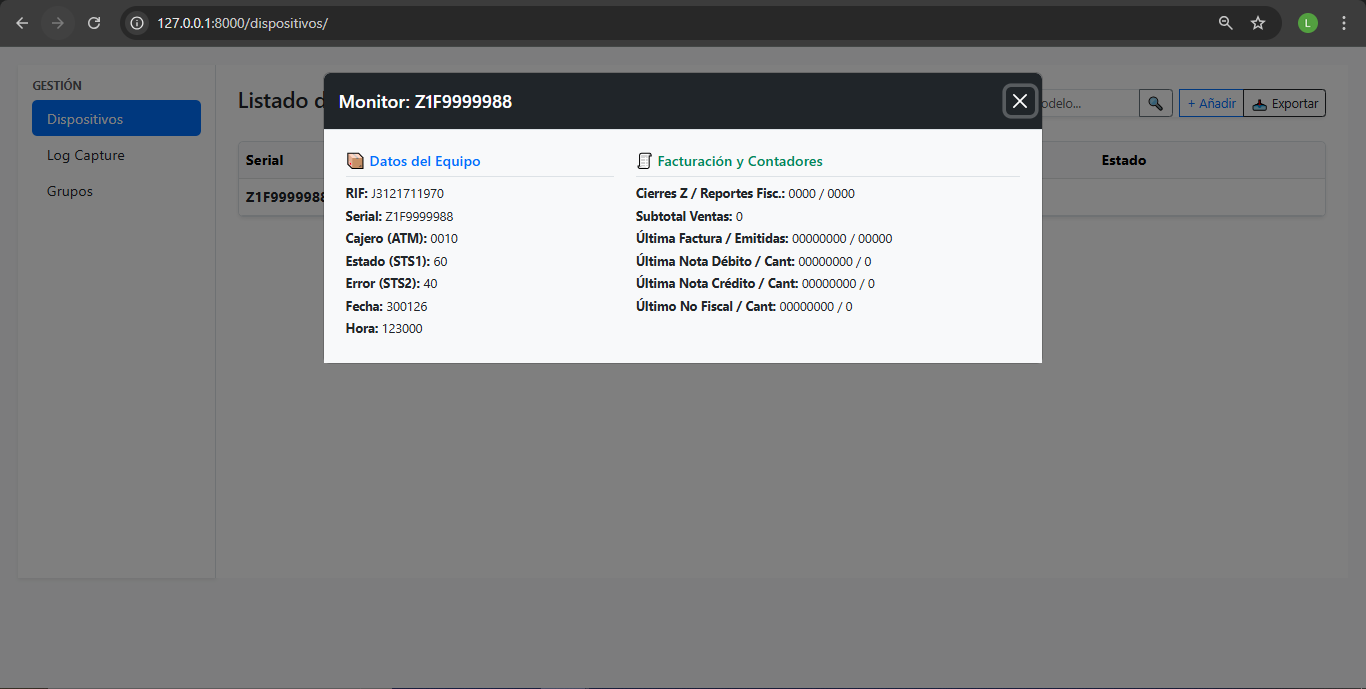
\includegraphics[width=0.9\linewidth]{Img/image31.png}
        \caption{Muestra de datos para impresora fiscal (simulada) mediante protocolo MQTT.}
        \label{fig:placeholder}
    \end{figure}

    \subsection*{Dificultades}

    \subsection*{Notas}

    \section*{Fecha: 20/02/2026}

    \subsection*{Actividades}

    \begin{itemize}
        \item Agregar seccion para eliminar dispositivos o administrar dispositivo.
        \item Implementar 'Estado' en Gestion de dispositivos.
        \item Implementar 'Grupo' en Gestion de dispositivos.
        \item Mejorar implementación de 'Modelo' en Gestion de dispositivos.
        \item Implementar botón 'Exportar'
        \item Implementar 'Log Capture'
    \end{itemize}

    \subsection*{Aprendizajes}

    Se implemento un sistema visual para conocer si la impresora esta en línea o si presenta algun error

    \begin{figure} [H]
        \centering
        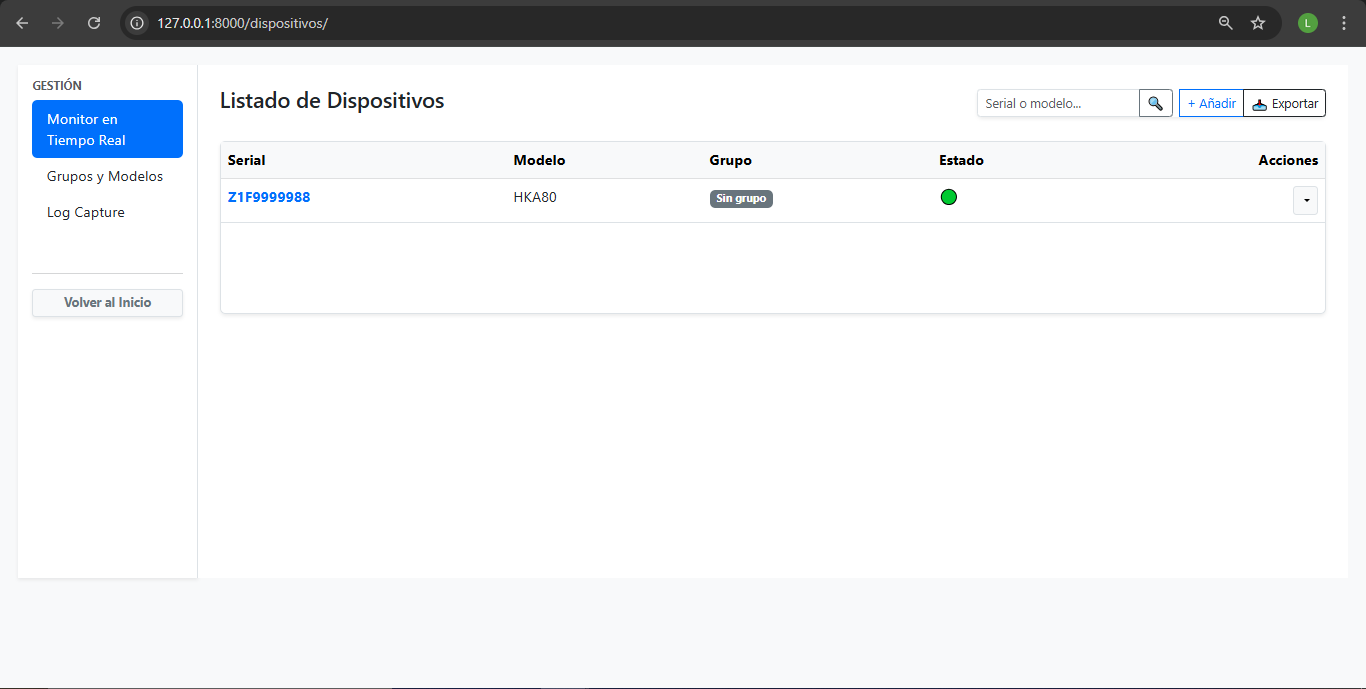
\includegraphics[width=0.9\linewidth]{Img/image32.png}
        \caption{Impresora en estado activo y recibiendo datos MQTT.}
        \label{fig:placeholder}
    \end{figure}

    \begin{figure} [H]
        \centering
        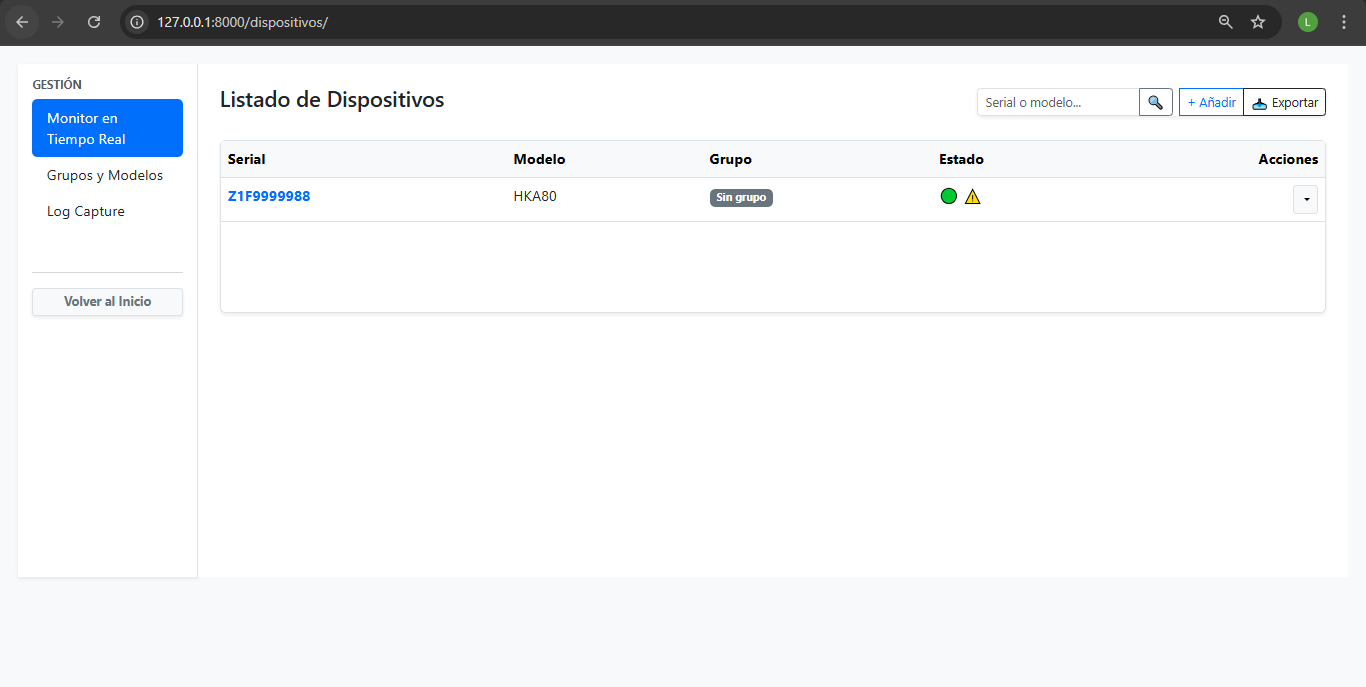
\includegraphics[width=0.9\linewidth]{Img/image36.png}
        \caption{Impresora que presenta un error y se encuentra en línea.}
        \label{fig:placeholder}
    \end{figure}

    Tambien se aplicaron modificaciones visuales a la visualizacion de datos, como la interpretación de STS1 y STS2, la visualizacion de fecha y hora, y el subtotal de ventas:
    
    \begin{figure} [H]
        \centering
        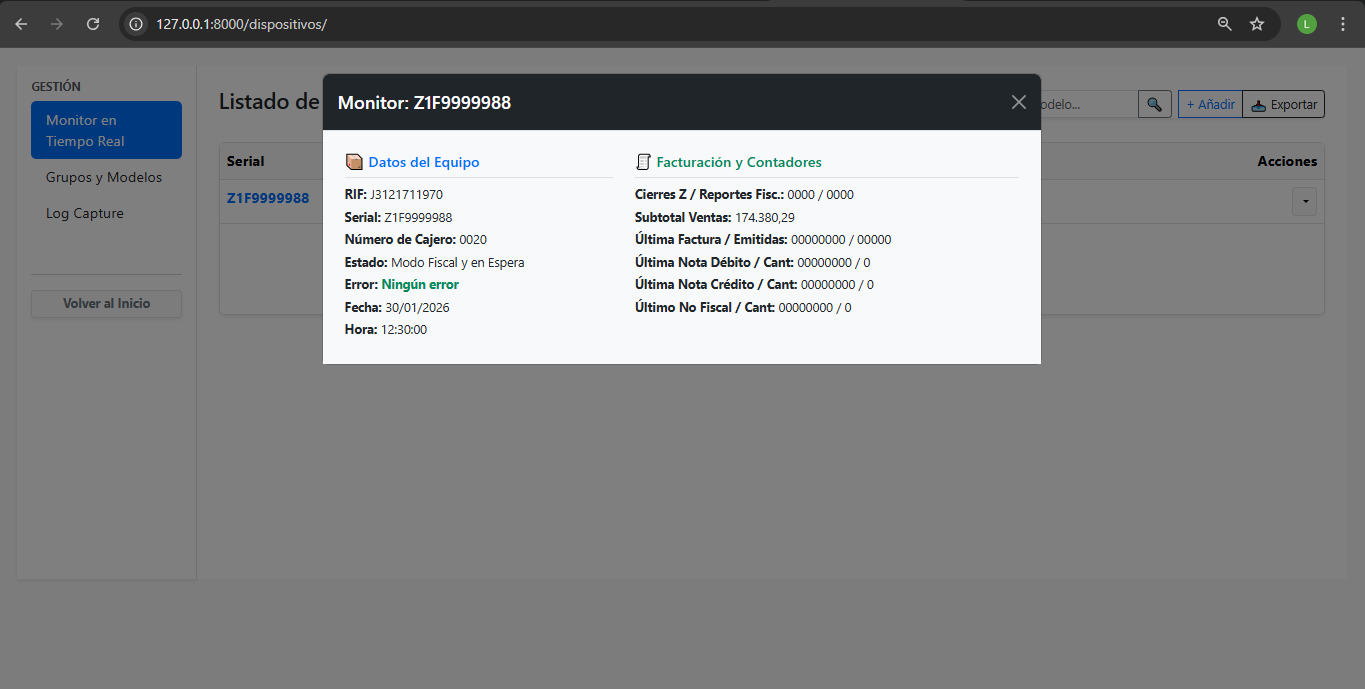
\includegraphics[width=0.9\linewidth]{Img/image33.png}
        \caption{Muestra de visualización de datos.}
        \label{fig:placeholder}
    \end{figure}

    Por otro lado se implemento la administración y visualización de los grupos y modelos que se pueden crear para el registro de una impresora:

    \begin{figure} [H]
        \centering
        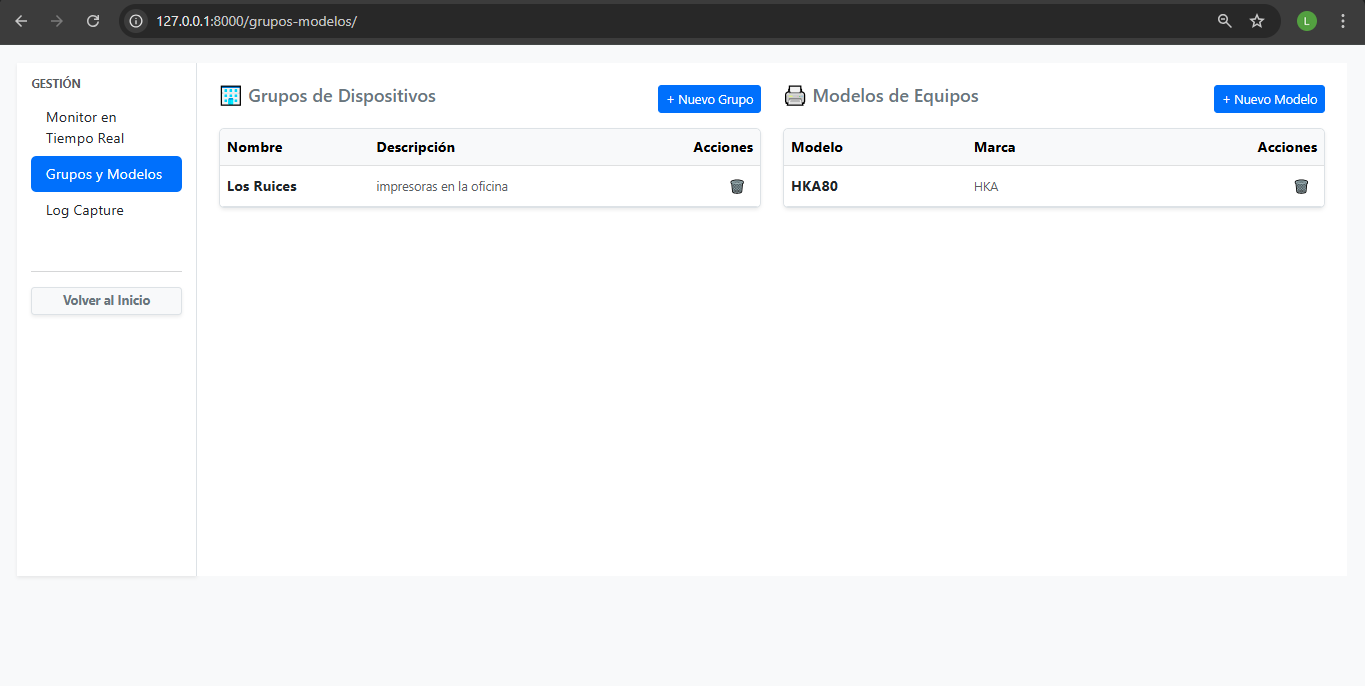
\includegraphics[width=0.9\linewidth]{Img/image34.png}
        \caption{Panel de 'Grupos y Modelos'.}
        \label{fig:placeholder}
    \end{figure}

    Finalmente, se implemento el log capture donde se pueden observar cambios de estado de un equipo asi la pagina no este abierta. Esto se logró mediante un worker que trabaja totalmente independiente de el server de la web, por lo cual se encuentra siempre registrando, y cualquier cambio se podrá observar mediante Log Capture.

    \begin{figure} [H]
        \centering
        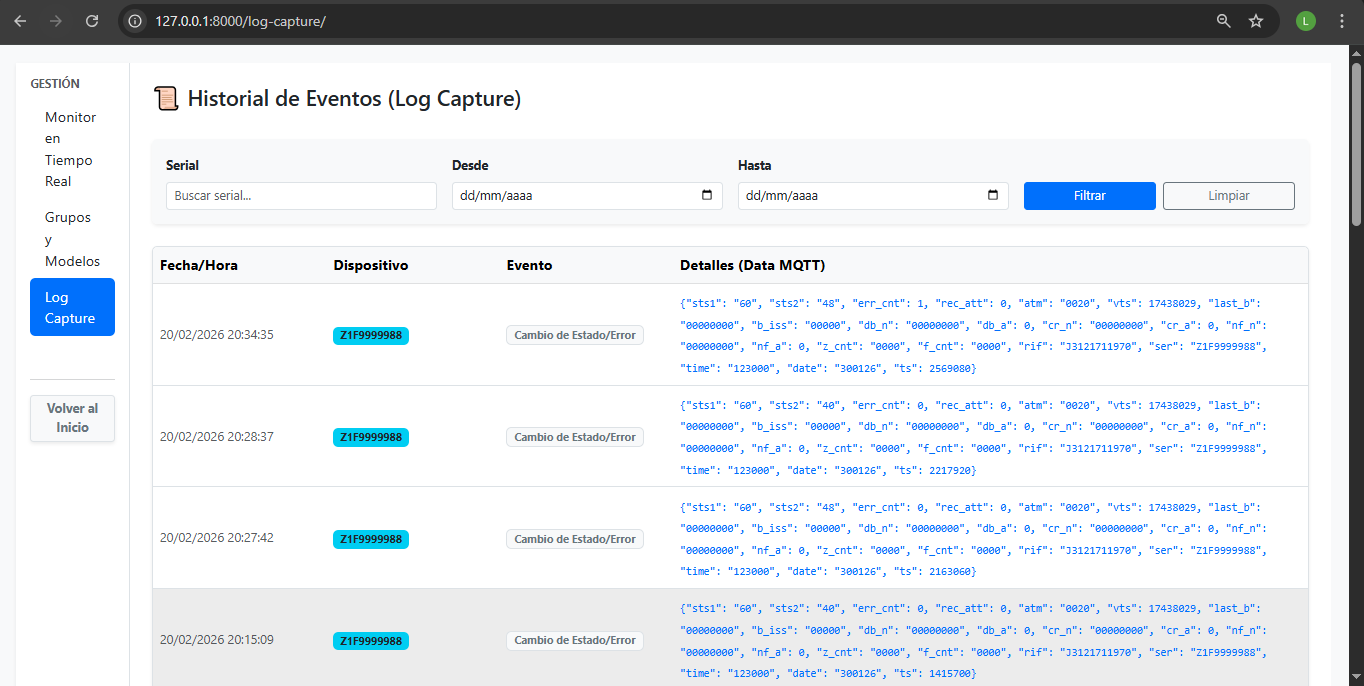
\includegraphics[width=0.9\linewidth]{Img/image37.png}
        \caption{Muestra de registro a cambio de error, de 0x40 a 0x48.}
        \label{fig:placeholder}
    \end{figure}

    \subsection*{Dificultades}

    \subsection*{Notas}

    \section*{Fecha: 23/02/2026}

    \subsection*{Actividades}

    \begin{itemize}
        \item Terminar de arreglar botón de 'limpiar' en log capture.
        \item Comenzar a implementar 'Gestión de Firmware'.
        \item Con "Gestión de Dispositivos" culminado, mejorar la visualización del Dashboard.
    \end{itemize}

    \subsection*{Aprendizajes}

    Avanzando con el desarrollo web, y cumpliendo con los objetivos pautados. Se realizo una mejor implmentacion para 'Log Capture', donde el usuario puede buscar por serial el historial de los ultimos 90 días para la impresora en cuestion.

    \begin{figure} [H]
        \centering
        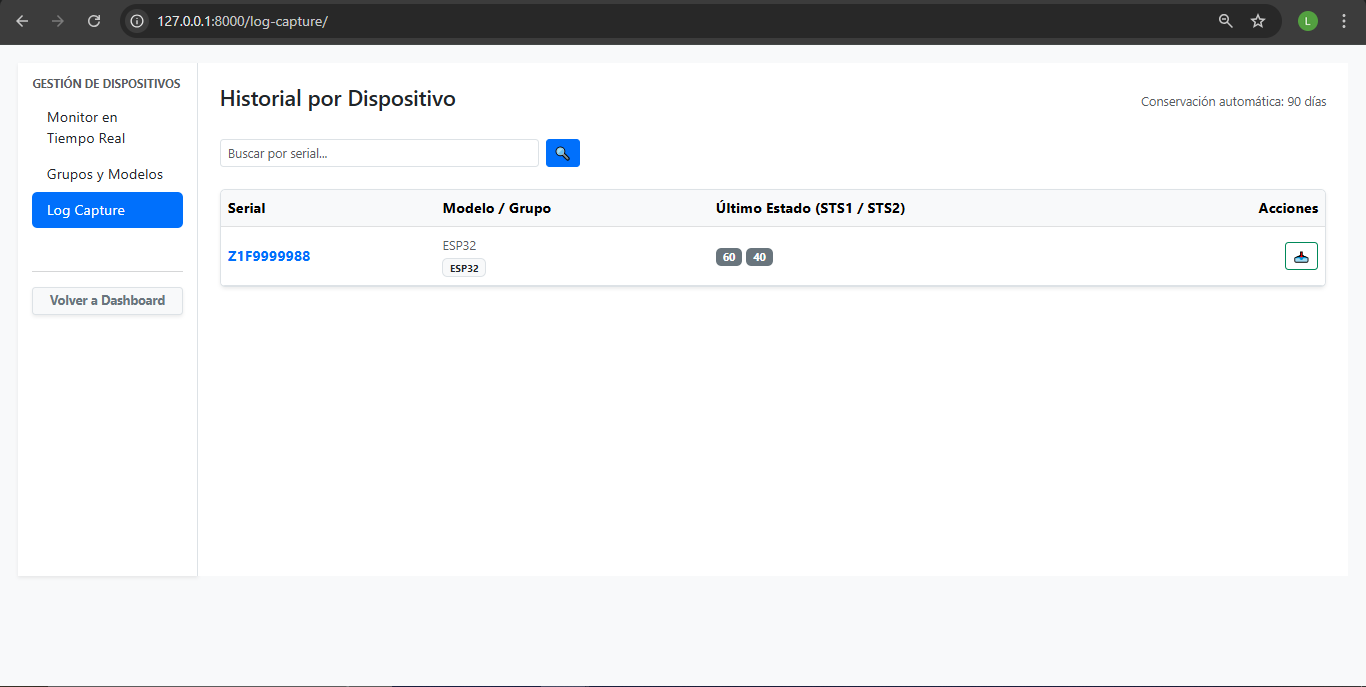
\includegraphics[width=0.9\linewidth]{Img/image38.png}
        \caption{Visualizacion para 'Log Capture'.}
        \label{fig:placeholder}
    \end{figure}

    Haciendo click en el serial del dispositivo a indagar, podemos ver los ultimos cambios de estado o cambios de error que realizó.

    \begin{figure} [H]
        \centering
        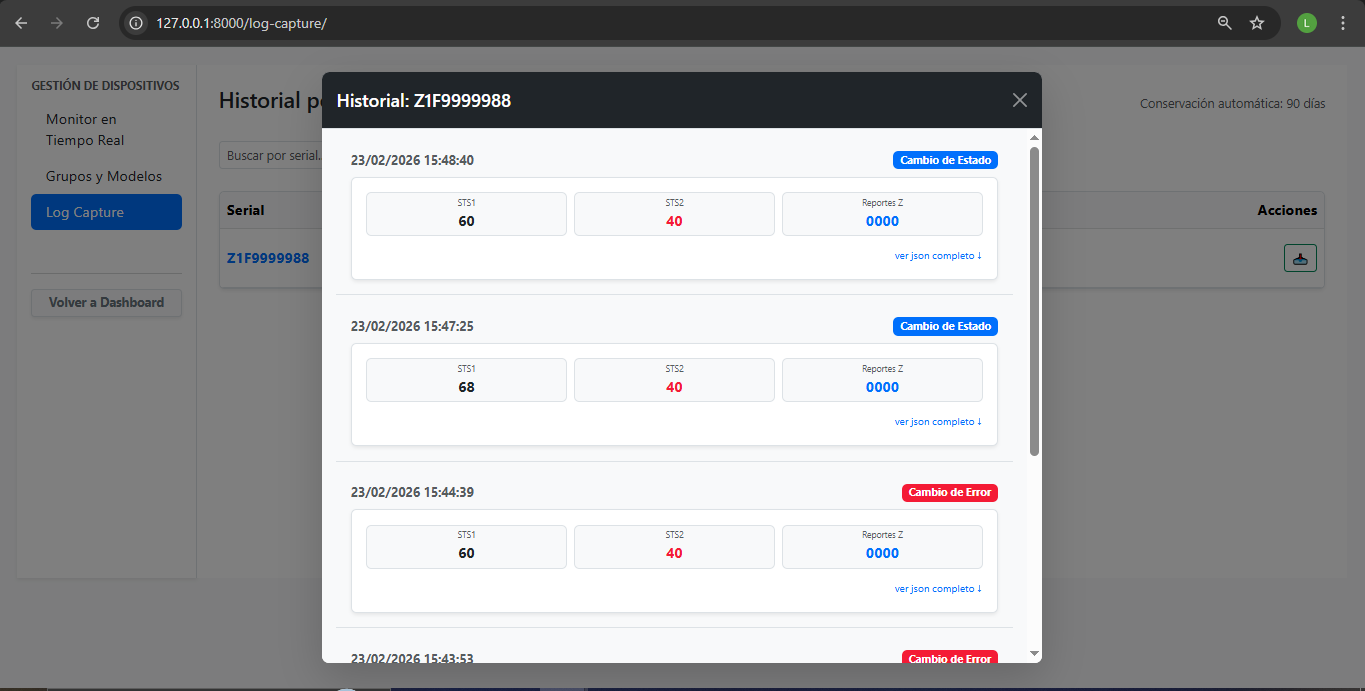
\includegraphics[width=0.9\linewidth]{Img/image39.png}
        \caption{Muestra de los ultimos cambios para el dispositivo prueba 'Z1F9999988'.}
        \label{fig:placeholder}
    \end{figure}

    Por otro lado, se realizó un cambio de imagen para el dashboard principal, el cual ya puede tomar datos de 'Gestión de Dispositivos' y mostrar información resumida del mismo.

    \begin{figure} [H]
        \centering
        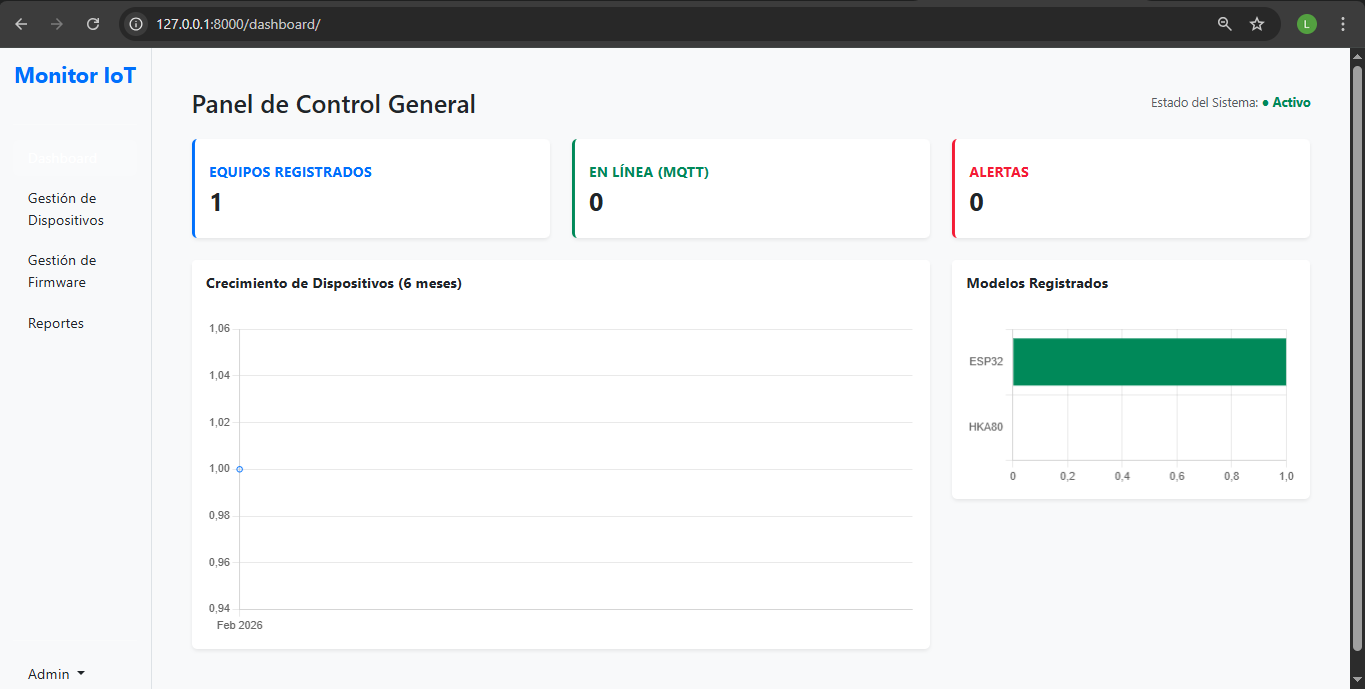
\includegraphics[width=0.9\linewidth]{Img/image40.png}
        \caption{Nuevo 'dashboard' principal con gráficos incluidos.}
        \label{fig:placeholder}
    \end{figure}

    Tambien se avanzó en la implementacion de 'Gestión de Firmware' donde se podrá subir las versiones nuevas de firmware para el isamrt.

    \begin{figure} [H]
        \centering
        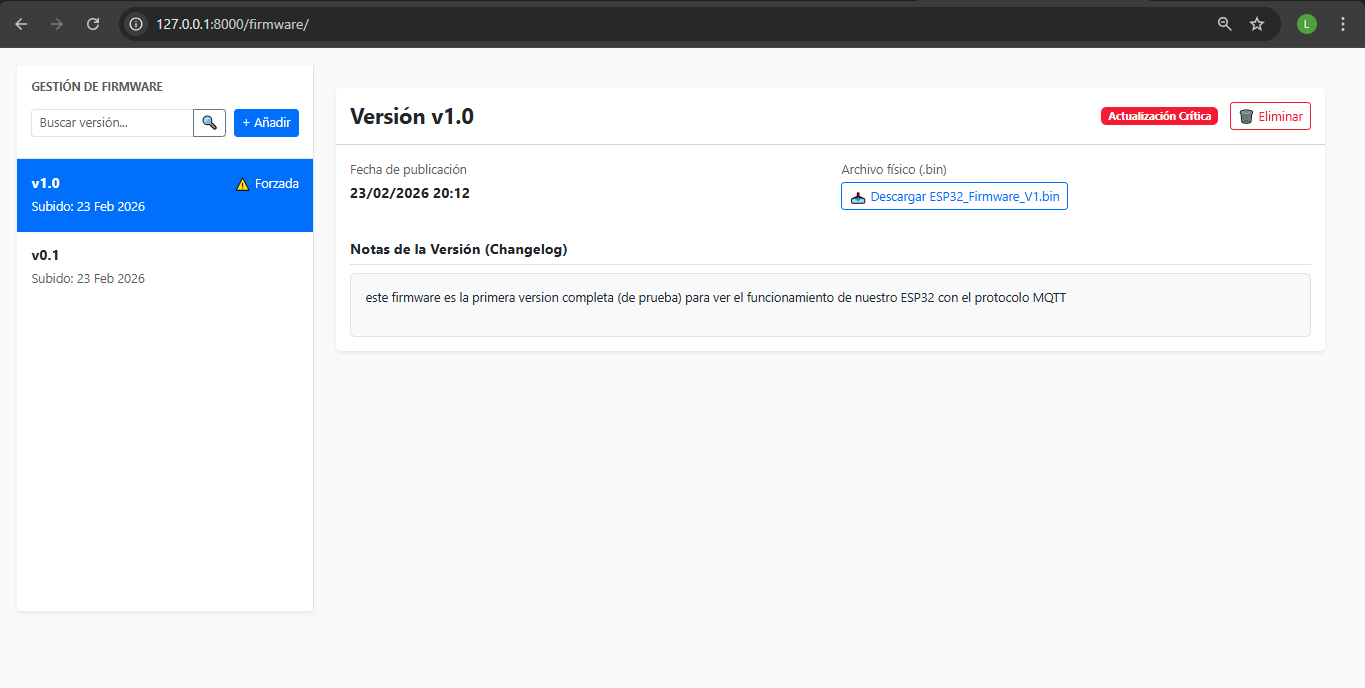
\includegraphics[width=0.9\linewidth]{Img/image41.png}
        \caption{Visualización para 'Gestión de Firmware' con archivos prueba publicados.}
        \label{fig:placeholder}
    \end{figure}

    \begin{figure} [H]
        \centering
        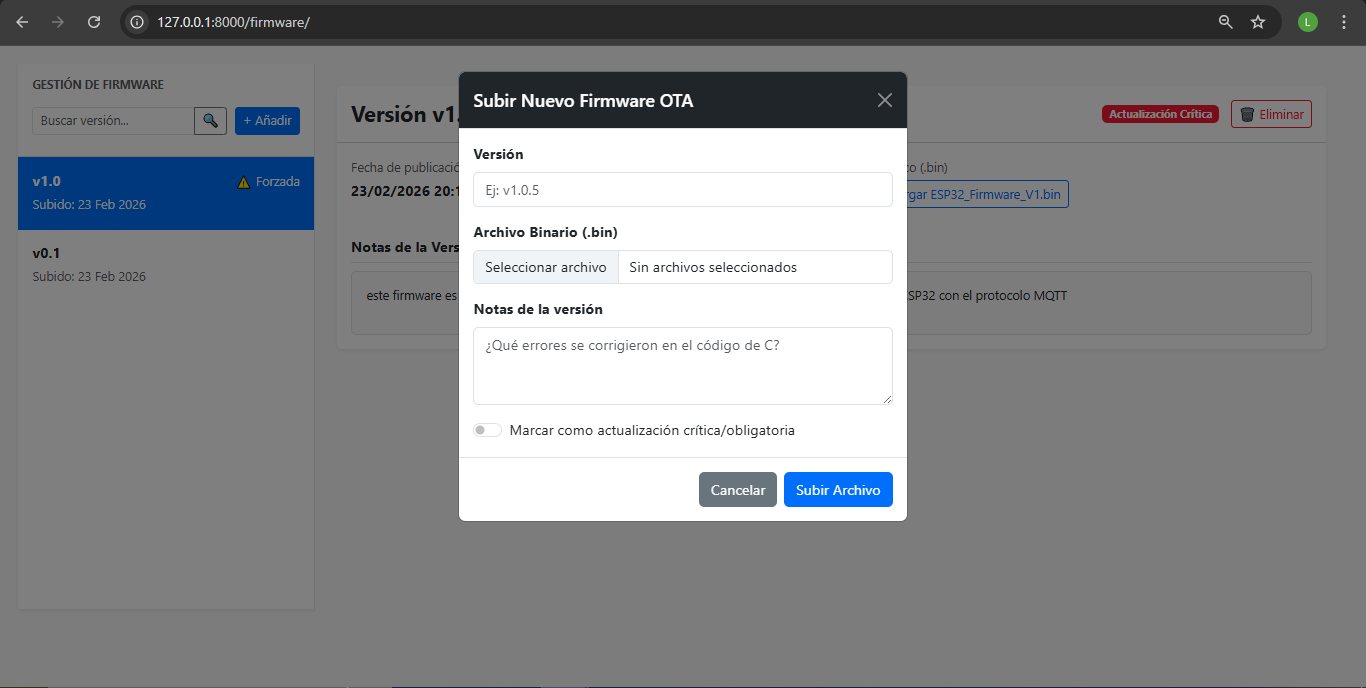
\includegraphics[width=0.9\linewidth]{Img/image42.png}
        \caption{Muesta para la adición de firmware nuevo.}
        \label{fig:placeholder}
    \end{figure}

    Y se incluyó un nuevo boton para actualizar el dispositivo en 'Gestion de Dispositivos'

    \begin{figure} [H]
        \centering
        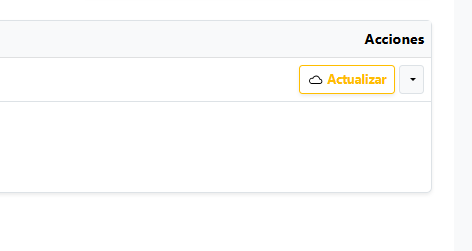
\includegraphics[width=0.9\linewidth]{Img/image43.png}
        \caption{Nuevo botón en las acciones de 'Gestión de Dispositivos'.}
        \label{fig:placeholder}
    \end{figure}

    \begin{figure} [H]
        \centering
        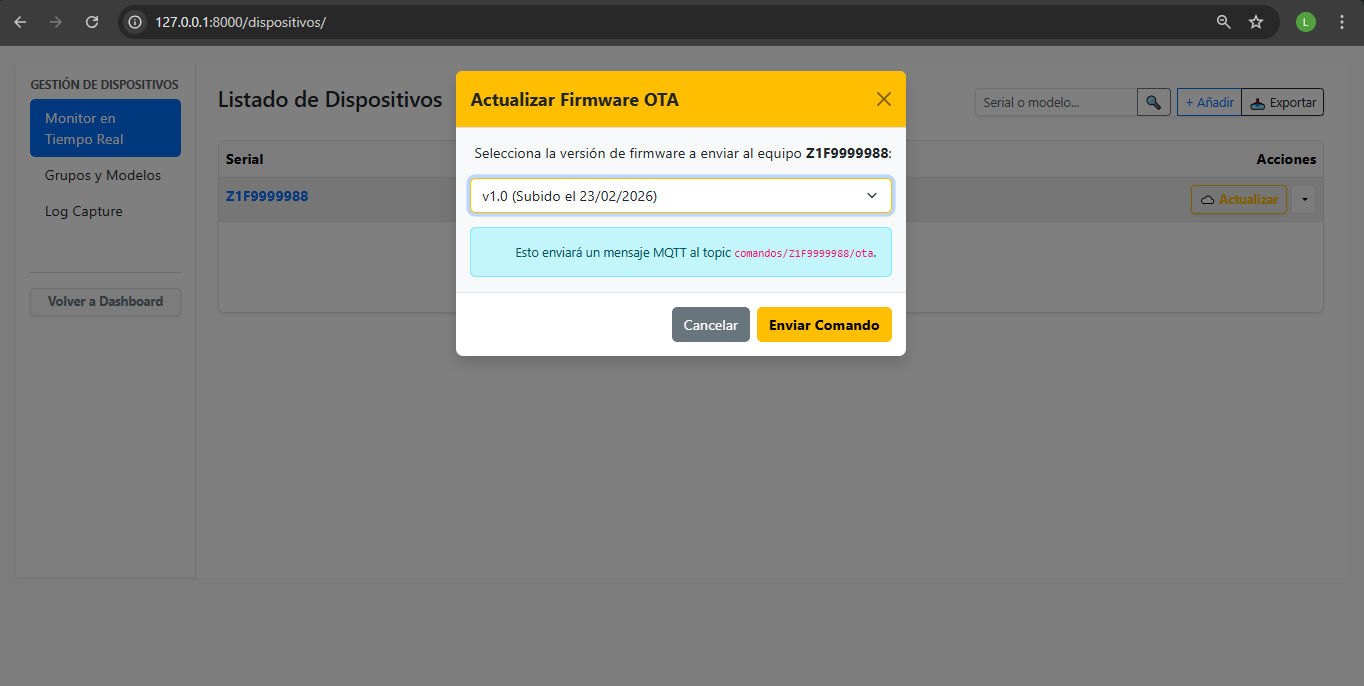
\includegraphics[width=0.9\linewidth]{Img/image44.png}
        \caption{Muestra para el menú de actualización de firmware.}
        \label{fig:placeholder}
    \end{figure}

    Dicho botón es estatico pero lo ideal es que sea dinamico, de forma que sirva como un anuncio de que el dispositivo necesita actualizarce.

    \subsection*{Dificultades}

    \subsection*{Notas}

    \section*{Fecha: 24/02/2026}

    \subsection*{Actividades}

    \begin{itemize}
        \item Hacer botón de 'Actualización' dinamico en 'Gestión de Dispositivos'.
        \item Mejorar repositorio de firmware en la web.
        \item Enviar mensaje MQTT desde la web al broker sobre actualización.
        \item Recibir mensaje MQTT del broker en el ESP32 para actualizar.
    \end{itemize}

    \subsection*{Aprendizajes}

    Hoy se culminó el desarrollo de la interfaz web, comenzando primero con la mejora del boton de actualización que estará disponible en todos los dispositivos registrados.

    \begin{figure} [H]
        \centering
        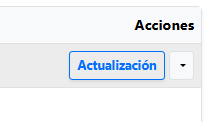
\includegraphics[width=0.5\linewidth]{Img/image46.png}
        \caption{Mejora de botón para visualizar menú de actualización.}
        \label{fig:placeholder}
    \end{figure}

    Donde en el mismo se podrá visualizar la versión del modulo de transmisión y de la impresora conectada al modulo de transmisión:

    \begin{figure} [H]
        \centering
        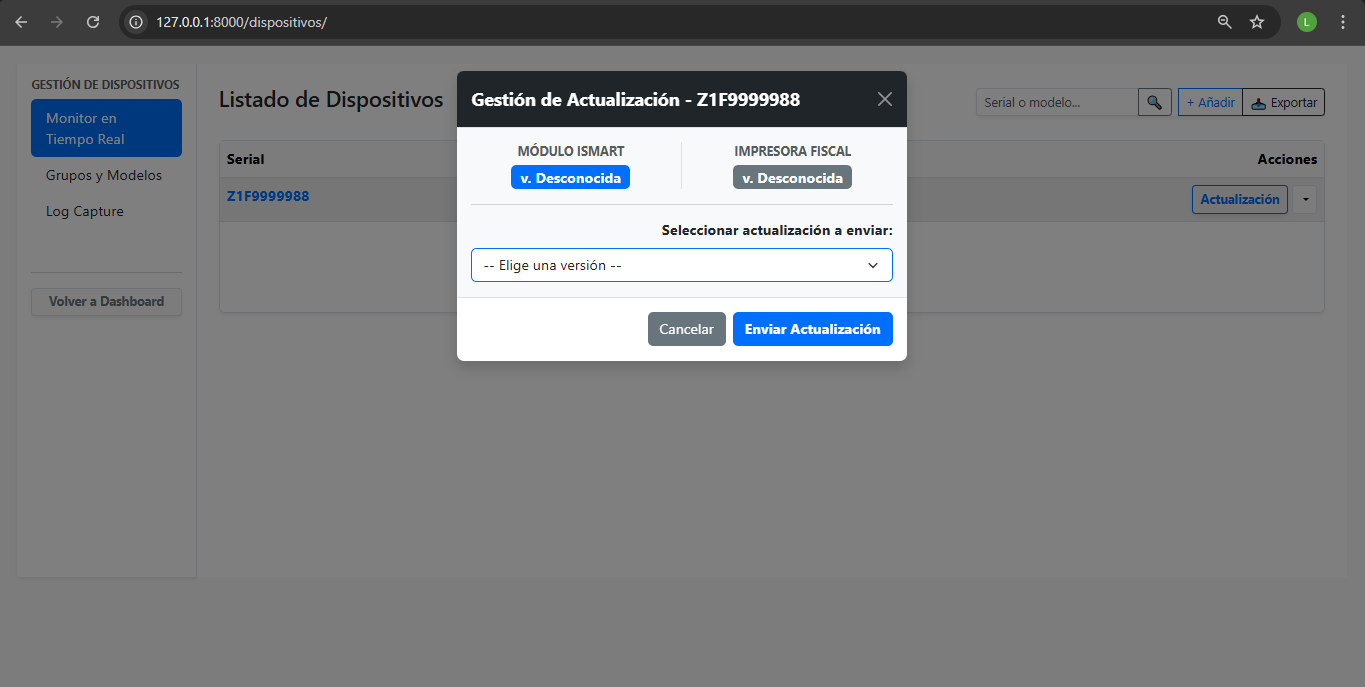
\includegraphics[width=0.9\linewidth]{Img/image47.png}
        \caption{Menú de actualización disponible en la interfaz.}
        \label{fig:placeholder}
    \end{figure}

    \textit{Nota:} Las versiones para el dispositivo resgistrado no se encuentran disponible porque falta actualizar el json que envia nuestro ESP32 con estos nuevos datos.

    Por otro lado, tambien se mejoro el repositorio de firmware hecho el dia anterior, ya que es necesario manejar diferentes versiones de diferentes firmware.

    \begin{figure} [H]
        \centering
        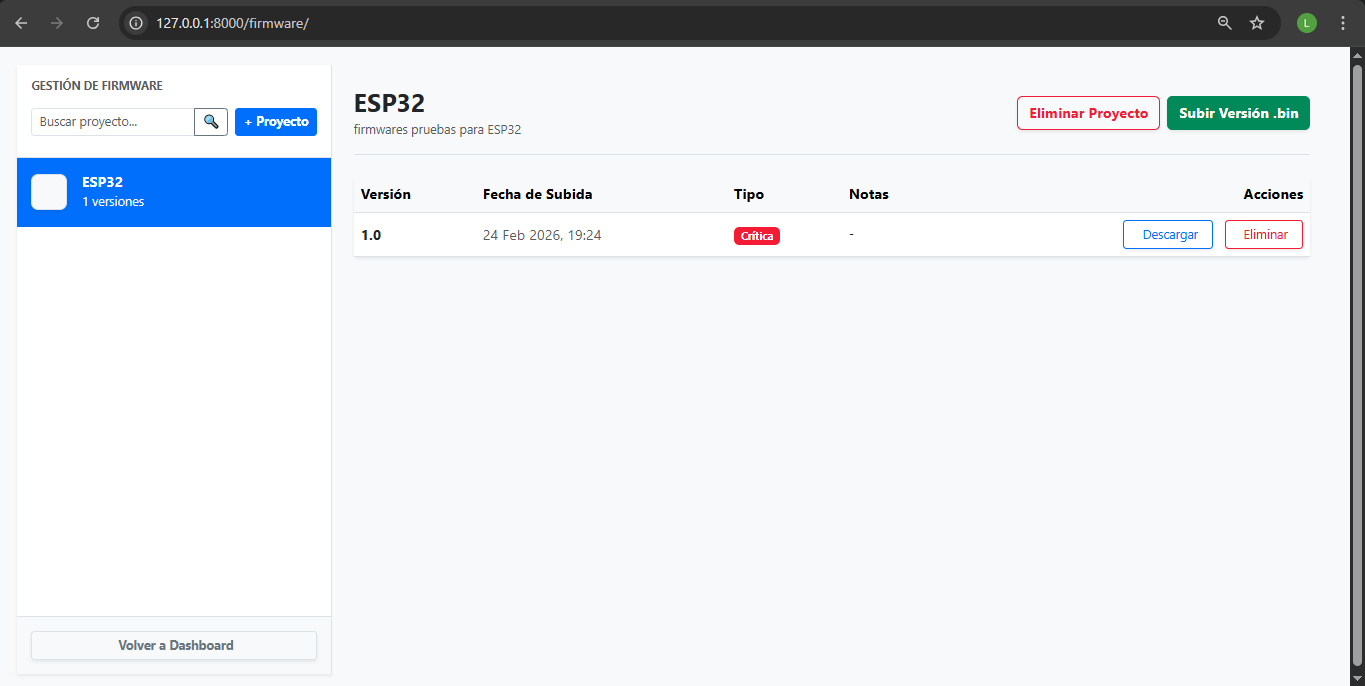
\includegraphics[width=0.9\linewidth]{Img/image48.png}
        \caption{Nueva interfaz para 'Gestión de Firmware'.}
        \label{fig:placeholder}
    \end{figure}

    Aqui ahora podemos añadir proyectos y dentro de los proyectos subir las nuevas versiones disponibles. Y con todos estos cambios vemos que es posible enviar mensajes MQTT en el broker de HiveMQ Cloud.

    \begin{figure} [H]
        \centering
        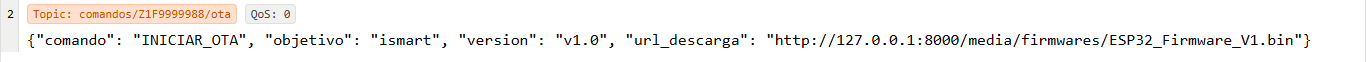
\includegraphics[width=0.9\linewidth]{Img/image45.png}
        \caption{Mensaje de actualización enviado al broker con objetivo de llegar al ESP32.}
        \label{fig:placeholder}
    \end{figure}

    \subsection*{Dificultades}

    \subsection*{Notas}

    Falto culminar la recepción en el ESP32 del broker para culminar el protocolo OTA, pero en vista que tambien hay que modificar el firmware para enviar las versiones los objetivos se aplazaron para el dia siguiente.

    \section*{Fecha: 25/02/2026}

    \subsection*{Actividades}

    \begin{itemize}
        \item Recibir comando S3 en nuestro ESP32.
        \item Enviar el nuevo formato JSON con las versiones de firmware.
        \item Recibir mensaje MQTT para actualización OTA.
    \end{itemize}

    \subsection*{Aprendizajes}

    Por instrucción de Luis, se tomo la desición de usar el envio de comando 'SV2' para conseguir la versión del firmware de la impresora. Por lo tanto, aplicando las modificaciones ahora nuestro formato JSON que enviamos por protocolo MQTT muestra las versiones tanto de nuesto ESP32 (iSmart) como el de nuestra impresora fiscal.

    \begin{figure} [H]
        \centering
        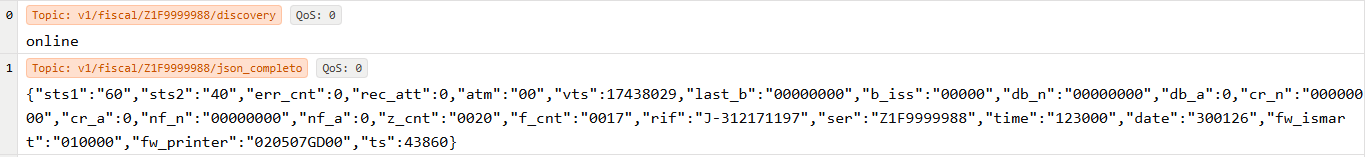
\includegraphics[width=1\linewidth]{Img/image49.png}
        \caption{Nuevo formato JSON funcional para actualizaciones OTA.}
        \label{fig:placeholder}
    \end{figure}

    Por otro lado, se trabaja en la actualización OTA en el caso del firmware de nuestro ESP32, para luego avanzar en el manejo del protocolo SPI y actualizar la impresora fiscal.

    \subsection*{Dificultades}

    \subsection*{Notas}

    \section*{Fecha: 27/02/2026 (Viernes)}

    \subsection*{Actividades}

    \begin{itemize}
        \item Adaptar nuevo formato de 'versión' en la visualización de la web.
        \item Arreglar errores de compilación para libreria http.
        \item Reunión con Pablo para enseñar avances.
        \item Arreglar horas en la web a horas locales de Venezuela.
    \end{itemize}

    \subsection*{Aprendizajes}

    \subsection*{Dificultades}

    \subsection*{Notas}

    \section*{Fecha: 02/03/2026}

    \subsection*{Actividades}

    \begin{itemize}
        \item Lograr actualización OTA en ESP32.
        \item Iniciar código para actualización de impresora fiscal.
        \item Modificar Log Capture para guardar cambios en versiones.
        \item Corregir errores em \texttt{listen\_mqtt}.
    \end{itemize}

    \subsection*{Aprendizajes}

    {\color{red} \subsubsection*{Configuración para optimizar uso de IRAM}}

    \begin{figure} [H]
        \centering
        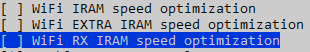
\includegraphics[width=0.5\linewidth]{Img/image50.png}
        \caption{Desactivamos arranque de WiFi con IRAM.}
        \label{fig:placeholder}
    \end{figure}

    {\color{red} \subsubsection*{Configuración para lograr actualización OTA}}

    \begin{figure} [H]
        \centering
        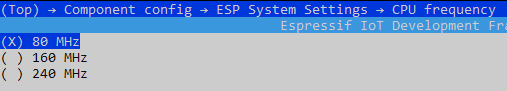
\includegraphics[width=0.7\linewidth]{Img/image51.png}
        \caption{Bajamos la frecuencia de reloj para evitar alto consumo de energía.}
        \label{fig:placeholder}
    \end{figure}

    \begin{figure} [H]
        \centering
        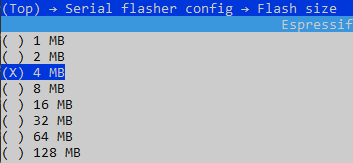
\includegraphics[width=0.7\linewidth]{Img/image52.png}
        \caption{Configuramos el 'Flash size' en 4MB para que haya suficiente espacio para la actualización.}
        \label{fig:placeholder}
    \end{figure}

    \begin{figure} [H]
        \centering
        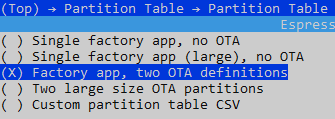
\includegraphics[width=0.7\linewidth]{Img/image53.png}
        \caption{En la tabla de particiones habilitamos la opción para dos definiciones OTA.}
        \label{fig:placeholder}
    \end{figure}

    \subsection*{Dificultades}

    \subsection*{Notas}

    \section*{Fecha: 03/03/2026}

    \subsection*{Actividades}

    \begin{itemize}
        \item Mejorar sistema de actualización en la web, con alertas y visualización de actualización critica.
        \item Continuar con código para actualizar impresora fiscal.
        \item Hacer cambio de comprador.
    \end{itemize}

    \subsection*{Aprendizajes}

    {\color{red} \subsubsection*{Mejoras en el modal de actualización en la pagina web}}

    \begin{figure} [H]
        \centering
        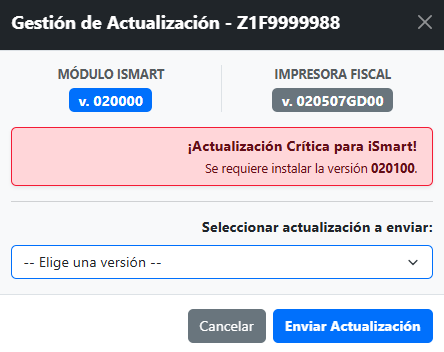
\includegraphics[width=0.5\linewidth]{Img/image54.png}
        \caption{Nueva advertencia visual cuando existe una actualización pendiente obligatoria.}
        \label{fig:placeholder}
    \end{figure}

    \begin{figure} [H]
        \centering
        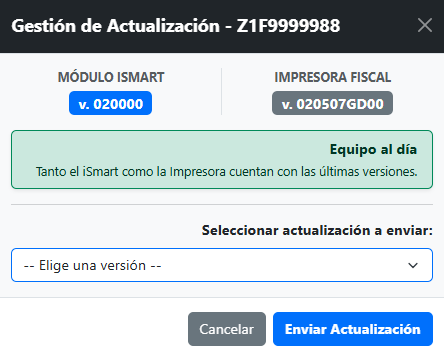
\includegraphics[width=0.5\linewidth]{Img/image55.png}
        \caption{Nueva advertencia visual que asegura cuando el equipo tiene las ultimas versiones instaladas.}
        \label{fig:placeholder}
    \end{figure}

    \subsection*{Dificultades}

    \subsection*{Notas}

    \section*{Fecha: 04/03/2026}

    \subsection*{Actividades}

    \begin{itemize}
        \item Implementar protocolo de actualización en el ESP32 para la Impresora Fiscal.
        \item Verificar implementación de protocolo con Luis.
        \item Reformar web para mejorar conexión MQTT.
    \end{itemize}

    \subsection*{Aprendizajes}

    {\color{red} \subsubsection*{Protocolo de actualización}}

    Se implemento un protocolo de actualización el cual fue verificado y corregido por Luis, donde se comienza con un comando de inicio (en este caso 0x01), y esperamos un ACK por parte de la impresora.

    \begin{figure} [H]
        \centering
        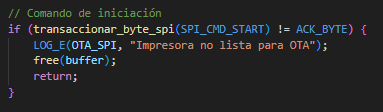
\includegraphics[width=0.6\linewidth]{Img/image56.png}
        \caption{Comando enviado a la impresora para iniciar proceso de actualización.}
        \label{fig:placeholder}
    \end{figure}

    Luego, nuestro ESP32 procede a enviar una trama de información que consiste en: Comando de paquete (0x02), número del paquete a enviar, cantidad de paquetes totales que enviaremos, tamaño de los datos en el paquete, datos del paquete y checksum. Luego, si el checksum es valido la impresora enviara un ACK.

    \begin{figure} [H]
        \centering
        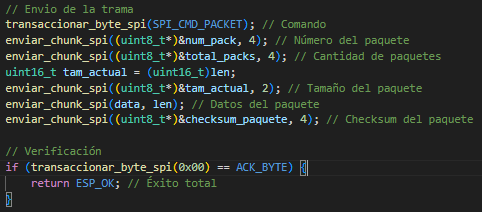
\includegraphics[width=0.6\linewidth]{Img/image57.png}
        \caption{Envio de la trama y respuesta ACK por parte de la impresora.}
        \label{fig:placeholder}
    \end{figure}

    Finalmente, luego de enviar todas las tramas, se envia un comando de culminación.

    \begin{figure}
        \centering
        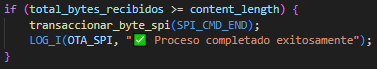
\includegraphics[width=0.6\linewidth]{Img/image58.png}
        \caption{Comando de finalización de actualización.}
        \label{fig:placeholder}
    \end{figure}

    {\color{red} \subsubsection*{Mejora de visualización en pagina web}}

    Se aplico un pequeño cambio en la visualización de la web, aplicando un arquitectura SPA con HTMX, donde ahora el broker MQTT esta conectado en cualquier parte de la web, logrando mayor fluidez en el uso de la misma.

    \begin{figure} [H]
        \centering
        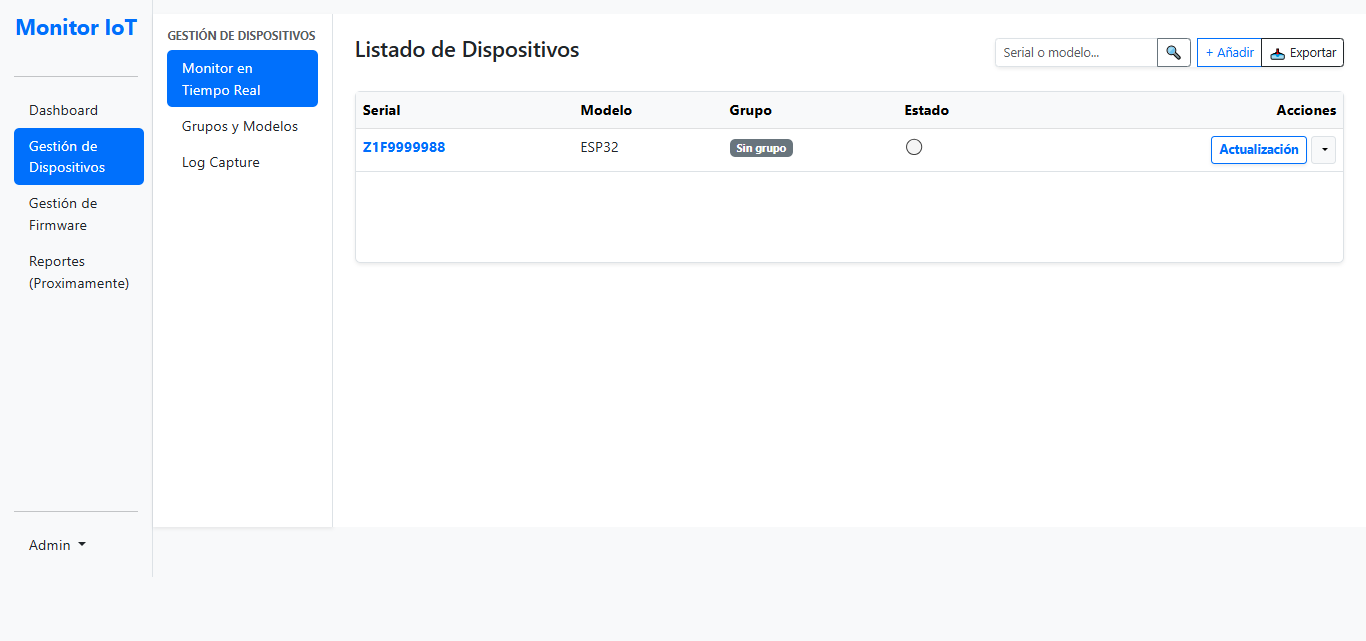
\includegraphics[width=0.9\linewidth]{Img/image59.png}
        \caption{Nueva perspectiva para la pagina web.}
        \label{fig:placeholder}
    \end{figure}
    
    \subsection*{Dificultades}

    \subsection*{Notas}

    \section*{Fecha: 06/03/2026 (Viernes)}

    \subsection*{Actividades}

    \begin{itemize}
        \item Implementar icono amarillo para cuando se actualice la impresora en la web.
        \item Generar aviso de impresora actualizada en la web.
    \end{itemize}

    \subsection*{Aprendizajes}

    {\color{red} \subsubsection*{Mejoras en el código firmware para seguimiento de actualización}}

    Con la implementación de una nueva función podremos ver como avanza la actualización tanto para el ESP32 como para la impresora, la cual llamamos en las diferentes tareas de actualización que maneja nuestro microcontrolador.
    
    \begin{figure} [H]
        \centering
        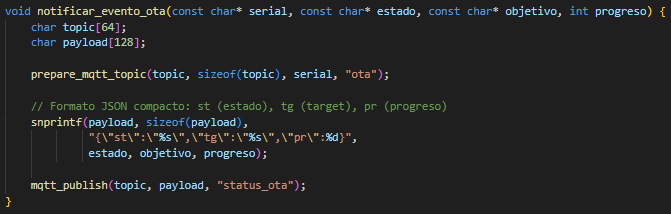
\includegraphics[width=0.7\linewidth]{Img/image60.png}
        \caption{Nueva función para notificar constantemente el proceso de actualización.}
        \label{fig:placeholder}
    \end{figure}

    {\color{red} \subsubsection*{Cambios a la interfaz WEB}}

    Se estudiaron los casos borde para evitar el error 404 de django a webs que antes no se habian especificado.

    \begin{figure} [H]
        \centering
        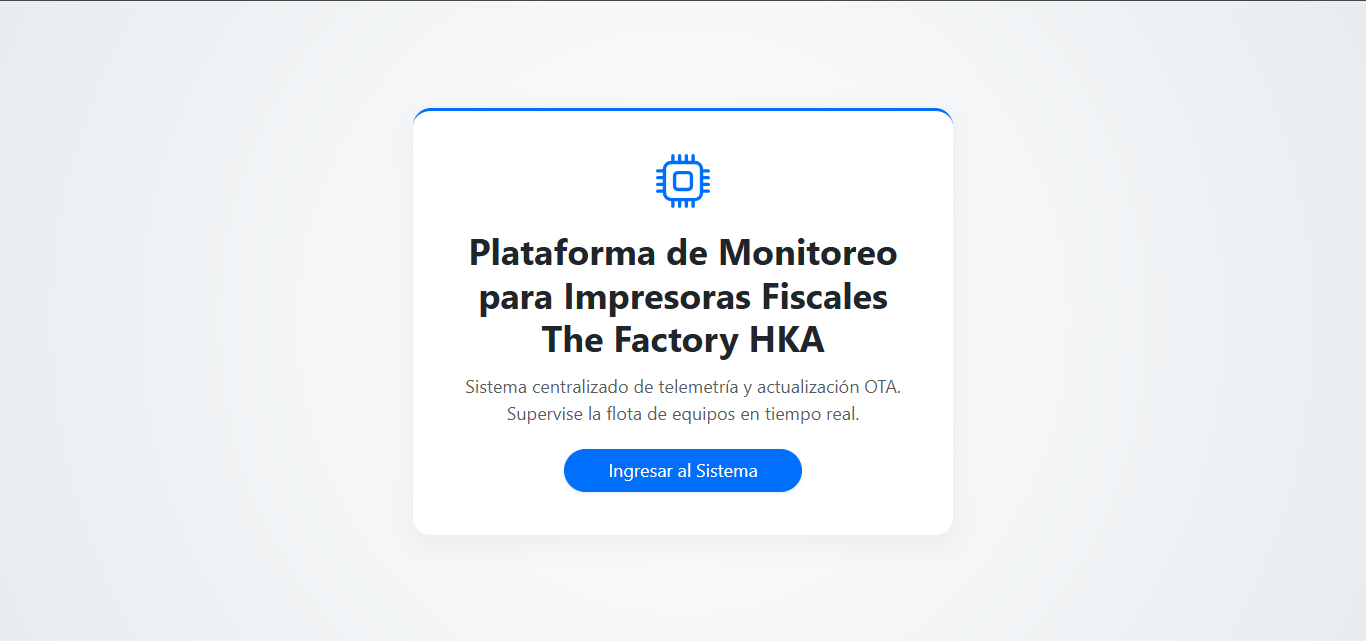
\includegraphics[width=0.9\linewidth]{Img/image61.png}
        \caption{Página de bienvenida al Sistema de Monitoreo.}
        \label{fig:placeholder}
    \end{figure}

    \begin{figure} [H]
        \centering
        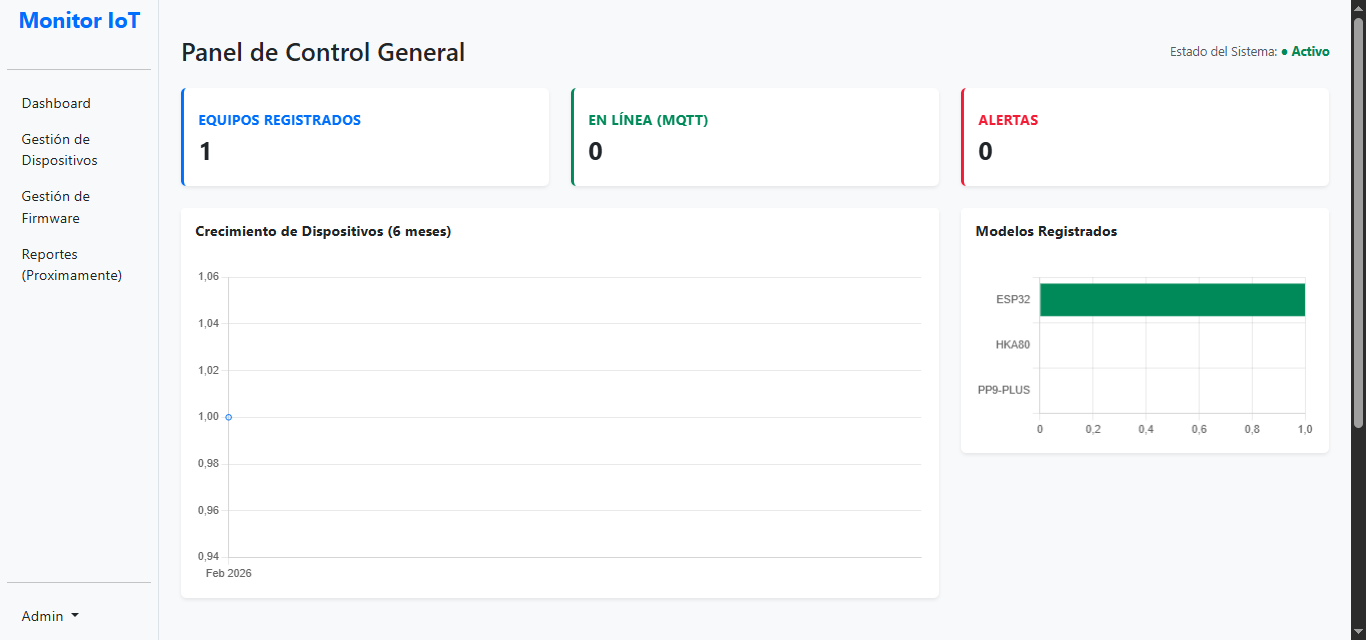
\includegraphics[width=0.9\linewidth]{Img/image62.png}
        \caption{Ligero cambio en panel izquierdo de la interfaz.}
        \label{fig:placeholder}
    \end{figure}

    \subsection*{Dificultades}

    \subsection*{Notas}

    \section*{Fecha: 06/03/2026}

    \subsection*{Actividades}

    \begin{itemize}
        \item Implementar porcentaje de actualización en el modal 'Gestión de actualización'.
        \item Corregir en su totalidad código firmware del ESP32.
    \end{itemize}

    \subsection*{Aprendizajes}

    \subsection*{Dificultades}

    \subsection*{Notas}

    \section*{Fecha: 10/03/2026}

    \subsection*{Actividades}

    \begin{itemize}
        \item Buscar y corregir inconsistencias en el sistema completo.
        \item Revisar lista de actividades en el area de hardware y desempeñar al menos una.
    \end{itemize}

    \subsection*{Aprendizajes}

    \subsection*{Dificultades}

    \subsection*{Notas}

    \section*{Fecha: 11/03/2026}

    \subsection*{Actividades}

    \begin{itemize}
        \item Elaborar guía de 'buenas prácticas de manejo de memoria en ESP-IDF'.
        \item Comenzar mi libro de pasantías.
    \end{itemize}

    \subsection*{Aprendizajes}

    \subsection*{Dificultades}

    \subsection*{Notas}

    \section*{Fecha: 12/03/2026}

    \subsection*{Actividades}

    \begin{itemize}
        \item Dejar todo instalado
        \item Hacer pruebas con al menos 2 dispositivos.
    \end{itemize}

    \subsection*{Aprendizajes}

    \subsection*{Dificultades}

    \subsection*{Notas}

    \section*{Fecha: 13/03/2026 (Viernes)}

    \subsection*{Actividades}

    \begin{itemize}
        \item Investigar sobre las buenas prácticas de diseño PCB.
        \item Instalar Altium Designer en el nuevo computador.
    \end{itemize}

    \subsection*{Aprendizajes}

    \subsection*{Dificultades}

    \subsection*{Notas}

    \section*{Fecha: 16/03/2026}

    \subsection*{Actividades}

    \begin{itemize}
        \item Correr proyecto de pasantías en la nueva laptop.
        \item Realizar pruebas de nuevas funcionalidades añadidas.
    \end{itemize}

    \subsection*{Aprendizajes}

    A este punto el proyecto se encuentra culminado y esta como pendiente añadir funcionalidades extras que mejoren la experiencia de usuario.

    \subsection*{Dificultades}

    \subsection*{Notas}

    \section*{Fecha: 18/03/2026}

    \subsection*{Actividades}

    \begin{itemize}
        \item Arreglar error de 'Alertas: 1'.
        \item En el nuevo cuadro de 'Calidad de conexión' generar aviso de 'desconexión'.
        \item Probar sistema con al menos 2 dispositivos.
    \end{itemize}

    \subsection*{Aprendizajes}

    \subsection*{Dificultades}

    \subsection*{Notas}

    \section*{Fecha: 19/03/2026}

    \subsection*{Actividades}

    \begin{itemize}
        \item Probar los programadores que me designo Pablo.
        \item Probar comunicación SPI.
        \item Añadir versiones fw\_ismart y fw\_printer al JSON de 'Desconexión abrupta'.
    \end{itemize}

    \subsection*{Aprendizajes}

    \subsection*{Dificultades}

    \subsection*{Notas}

    \section*{Fecha: 20/03/2026}

    \subsection*{Actividades}

    \begin{itemize}
        \item Ver lección 1 del modulo 1 del curso PCB.
        \item Actualizar bitacora de pasantías. 
    \end{itemize}

    \subsection*{Aprendizajes}

    \subsection*{Dificultades}

    \subsection*{Notas}

    \section*{Fecha: 23/03/2026}

    \subsection*{Actividades}

    \begin{itemize}
        \item Migrar código del ESP32 de UART a SPI.
        \item Probar proyecto con multiples dispositivos.
    \end{itemize}

    \subsection*{Aprendizajes}

    \subsection*{Dificultades}

    \subsection*{Notas}

    \section*{Fecha: 25/03/2026}

    \subsection*{Actividades}

    \begin{itemize}
        \item Probar simulador impresora por SPI.
        \item Ver lección 2 y 3 del modulo 1 del curso PCB.
    \end{itemize}

    \subsection*{Aprendizajes}

    \subsection*{Dificultades}

    \subsection*{Notas}

    Por cuestiones de salud se faltaron los dias miercoles 25, jueves 26 y viernes 27. 

    \section*{Fecha: 30/03/2026}

    \subsection*{Actividades}

    \begin{itemize}
        \item Ponerme al día con los objetivos anteriores antes no cumplidos.
    \end{itemize}

    \subsection*{Aprendizajes}

    \subsection*{Dificultades}

    \subsection*{Notas}

    Este día fue para retomar los puntos anteriores, como por ejemplo, lograr la comunicación 100\% mediante SPI en el firmware para el ESP32, lo cual al cabo de la tarde en la jornada se logró.

    \section*{Fecha: 31/03/2026}

    \subsection*{Actividades}

    \begin{itemize}
        \item Arreglar posibles errores de multiple conexiones en la web.
    \end{itemize}

    \subsection*{Aprendizajes}

    Con 4 ESP32 a la mano es posible conectar 3 dispositivos a la web, donde 1 de ellos es mediante protocolo SPI y los otros dos mediante UART, el ultimo ESP32 se adapto para convertirlo en una impresora fiscal que se conecta mediante SPI a otro ESP32 tipo iSmart.

    \subsection*{Dificultades}

    El broker MQTT muestra inconsistencias al tener multiples dispositivos transmitiendo, pero no ocurre todo el tiempo, igual se tomara en cuenta para cuando se prueben varios dispositivos conectados.

    \subsection*{Notas}

    Hoy tambien se continuo con el curso de Altium llegando al Modulo 2.

    \section*{Fecha: 01/04/2026 (Miercoles de Semana Santa)}

    \subsection*{Actividades}

    \begin{itemize}
        \item Resolver problema de broker MQTT, de conexión inestable.
        \item Adaptar conexiones WiFi diferentes en el ESP32 y actualizar sin afectarlo.
        \item Ver modulo 3 del curso de Altium.
    \end{itemize}

    \subsection*{Aprendizajes}

    \subsection*{Dificultades}

    Enfocando los objetivos de hoy para hacer una actualizacion OTA 100\% robusta se obtuvieron problemas de prioridades de tareas en cuanto al envio de este comando desde la web. No obstante, se logro mantener la actualización OTA como la tarea mas importante de todo el firmware.

    \begin{figure} [H]
        \centering
        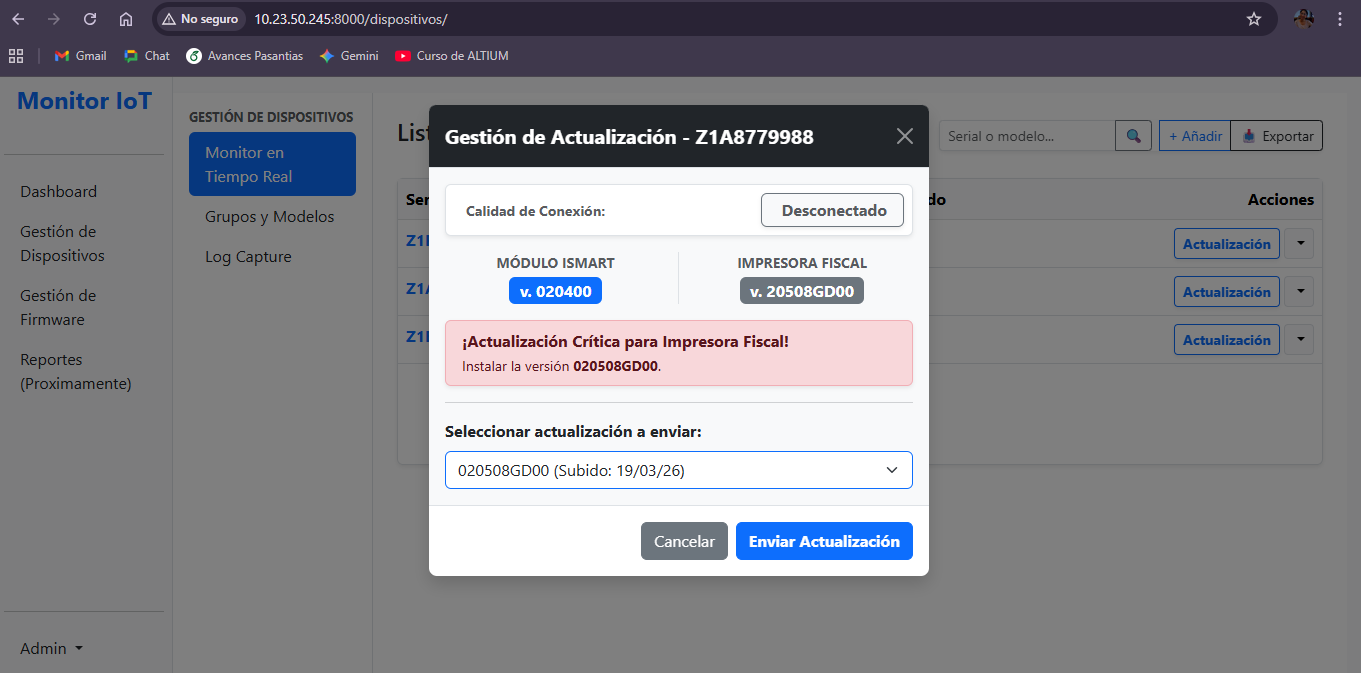
\includegraphics[width=0.9\linewidth]{Img/image63.png}
        \caption{Prueba de envio de comando para actualización.}
        \label{fig:placeholder}
    \end{figure}

    \begin{figure} [H]
        \centering
        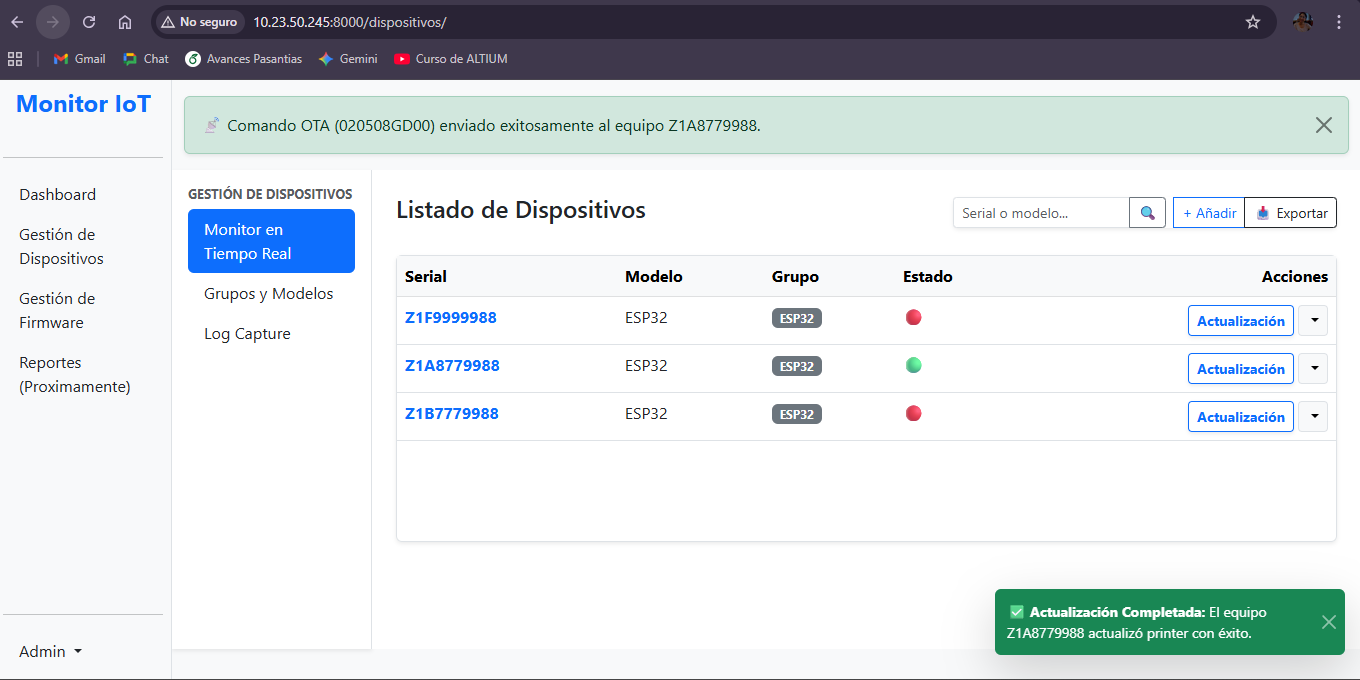
\includegraphics[width=0.9\linewidth]{Img/image64.png}
        \caption{Actualización hacia simulador de impresora completada satisfactoriamente a través de la web.}
        \label{fig:placeholder}
    \end{figure}

    \subsection*{Notas}

    \section*{Fecha: 06/04/2026}

    \subsection*{Actividades}

    \begin{itemize}
        \item Hacer revisión completa del sistema para elaborar documentación del funcionamiento.
    \end{itemize}

    \subsection*{Aprendizajes}

    {\color{red} \subsubsection*{Manejo de Errores y Robustez del Sistema (iSmart)}}
    
    Para garantizar la alta disponibilidad del nodo \textbf{iSmart}, se ha implementado una lógica de tolerancia a fallos estructurada en tres niveles de defensa:

    \begin{itemize}
        \item \textbf{Capa de Hardware (SPI):} Se implementaron \textit{timeouts} y mecanismos de limpieza de \textit{buffers}. Ante una trama corrupta, el firmware ejecuta una reinicialización del bus SPI (\texttt{spi\_bus\_free} y \texttt{spi\_bus\_initialize}), eliminando bloqueos por ruido electromagnético.
        
        \item \textbf{Protocolo de Reintentos (Regla de 3):} Se diseñó una máquina de estados que, ante una falla de lectura del estatus fiscal (S1), realiza hasta tres intentos con retardos incrementales. 
        
        \item \textbf{Resiliencia de Red (WiFi/MQTT):} Se configuró un modo de \textit{auto-reconnect} infinito. Adicionalmente, el estado del dispositivo se gestiona en memoria no volátil (NVS), permitiendo que el sistema retome su operación de forma autónoma tras reinicios inesperados o caídas de tensión.
    \end{itemize}

    \subsection*{Dificultades}

    {\color{red} \subsubsection*{Criterio para la configuración de conexión WiFi}}

    \begin{itemize}
        \item \textbf{Opción A: Software de Computadora (Estado Actual)} - El técnico conecta un cable Serial a la impresora fiscal, abre el programa en Windows, escribe el Wi-Fi y le da a 'Guardar'.

        \begin{itemize}
            \item Pros: 
            \begin{itemize}
                \item Ya está hecho.
                \item Es extremadamente seguro (requiere acceso físico al equipo).
                \item Es ideal para la 'Configuración en Laboratorio' (cuando preparan los equipos en las oficinas de HKA antes de mandarlos al cliente).
            \end{itemize}
            \item Contras:
            \begin{itemize}
                \item Si el Wi-Fi del cliente cambia la clave en el futuro, un tecnico tiene que ir físicamente con su equipo y reconfigurarlo.
            \end{itemize}
        \end{itemize}

        \item Opción B: El Portal Cautivo (La propuesta) - Si el equipo se queda sin Wi-Fi, levanta su propia red, el cajero o dueño de la tienda se conecta con su teléfono celular y pone la nueva clave.

        \begin{itemize}
            \item Pros:
            \begin{itemize}
                \item Cero cables y cero laptops.
                \item Autogestión: El mismo dueño del comercio puede cambiar el Wi-Fi si cambia de router, ahorrándole a The Factory HKA el costo de enviar a un técnico al sitio.
                \item Es el 'Estándar de la Industria' para dispositivos IoT modernos (como Alexa, bombillos inteligentes, etc.).
            \end{itemize}
            \item Contras:
            \begin{itemize}
                \item Requiere que le dedique un par de horas de programación extra en esta etapa final de tu proyecto.
            \end{itemize}
        \end{itemize}
    \end{itemize}
    
    \subsection*{Notas}

    \section*{Fecha: 07/04/2026}

    \subsection*{Actividades}

    \begin{itemize}
        \item Avanzar en la realización de la presentación de avances.
        \item Hacer pruebas de sistema activo.
        \item Avanzar en la redacción del informe de pasantías.
    \end{itemize}

    \subsection*{Aprendizajes}

    \subsection*{Dificultades}

    \subsection*{Notas}

    \section*{Fecha: 08/04/2026}

    \subsection*{Actividades}

    \begin{itemize}
        \item Solucionar error de desbordamiento ESP32 al actualizar.
        \item Mejorar lógica de actualización en \texttt{printer\_simulate}.
        \item Generar fotos y videos del sistema funcional.
        \item Ver video 3 del modulo 1.
        \item Terminar diapositivas.
    \end{itemize}

    \subsection*{Aprendizajes}

    {\color{red} \subsubsection*{Errores o bugs encontrados en el sistema}}

    
    \paragraph{Error 'Off-By-One' y el Carácter Invisible}
    
    Al enviar el JSON por MQTT, la versión de la impresora salía cortada y con basura al final (ej. 20507GD00 en lugar de 020507GD00). Esto ocurría porque la trama física de la impresora incluye un salto de línea (\n) justo antes del final (ETX). Al decirle al código "retrocede exactamente 10 pasos", agarraba ese \n invisible y dejaba por fuera el primer número.\\

    \textbf{La Solución:} Ajustamos la matemática restando un espacio extra (- 1) para esquivar exitosamente el salto de línea. Además, agregamos manualmente el terminador nulo (\0) al final del arreglo en RAM, garantizando que la librería que construye el JSON leyera un texto perfectamente limpio y cerrado.

    \paragraph{El Choque de Trenes SPI (Condición de Carrera en Hardware)}
    
    Al forzar una actualización OTA en el mismo milisegundo en que la tarea de la impresora enviaba un comando S1, ambas tareas intentaron adueñarse de los pines físicos del bus SPI a la vez. El controlador del hardware entró en pánico (assert failed) y reinició la placa para protegerse.\\

    \textbf{La Solución:} Implementamos un segundo Mutex de Hardware (\texttt{spi\_bus\_mutex}). Separamos la protección de los "datos en RAM" de la protección del "cable físico". Ahora, la tarea OTA y la tarea Fiscal hacen una fila ordenada para usar la antena SPI, evitando colisiones eléctricas.

    \paragraph{La Sordera Post-Actualización (Paradoja de Lógica y Tiempos)}
    
    Al reiniciarse el ESP32 tras un OTA (Soft Reset), la conexión Wi-Fi/MQTT se levantaba más rápido que la comunicación con la impresora. MQTT leía el serial como "DESCONOCIDO" y no se suscribía al tópico. Cuando la impresora por fin leía el serial real, el código sobrescribía la variable global antes de enviarla a la función de validación. La función comparaba el nuevo serial consigo mismo, creía que no había cambios, y jamás lanzaba la suscripción.\\

    \textbf{La Solución:} Eliminamos el copiado manual prematuro. Pasamos el dato recién leído (campos[13]) directamente a la función \texttt{update\_printer\_serial()}. Así, la función detecta el salto de "DESCONOCIDO" al serial real, activa la bandera, y fuerza la suscripción MQTT automáticamente en el momento correcto.

    \subsection*{Dificultades}

    \subsection*{Notas}

    {\color{red} \subsubsection*{Fallas que cubre exitosamente el sistema}}
    
    \paragraph{Resiliencia de Red y Conectividad (Wi-Fi & MQTT)}

    \begin{itemize}
        \item \textbf{Caídas Temporales de Wi-Fi:} Si el router se apaga o pierde señal, el sistema no se cuelga; entra en un ciclo de reconexión automática ('\texttt{WIFI\_EVENT\_STA\_DISCONNECTED}') hasta restablecer el enlace.
        \item \textbf{Bloqueos de DNS del ISP:} Si el proveedor de internet local tiene fallas de resolución de nombres, el firmware inyecta forzosamente los DNS de Google ('\texttt{8.8.8.8}') al obtener la IP, garantizando que siempre encuentre la ruta hacia el broker de HiveMQ.
        \item \textbf{Desconexiones de MQTT (Broker Drop):} Si el servidor MQTT expulsa al ESP32, la tarea entra en modo reposo ('\texttt{RECONNECT\_DELAY\_MS}') para no saturar la red, se reconecta y vuelve a suscribirse automáticamente al tópico correcto de OTA.
    \end{itemize}

    \paragraph{Tolerancia a Fallos Físicos y de Hardware (Bus SPI)}

    \begin{itemize}
        \item \textbf{Colisiones Eléctricas (El Choque de Trenes):} Si un comando OTA y un ciclo de monitoreo fiscal intentan hablar al mismo tiempo, el \textbf{Mutex de Hardware} ('\texttt{spi\_bus\_mutex}') actúa como un semáforo estricto. Impide que las señales eléctricas colisionen, evitando que el controlador SPI entre en pánico ('assert failed') y reinicie la placa.
        
        \item \textbf{Ruido Eléctrico y Tramas Corruptas:} Si la interferencia electromagnética altera un bit en el cable SPI, la función '\texttt{validate\_frame}' detecta la asimetría calculando el Checksum (LRC). Si no coincide, el ESP32 envía un NAK a la impresora y descarta la basura, protegiendo la integridad de la base de datos.

        \item \textbf{Impresora Apagada o Desconectada:} Si el cajero apaga la impresora físicamente, el ESP32 no se queda esperando infinitamente. Los \textbf{Timeouts estrictos} ('\texttt{esperar\_ack\_impresora}') abortan la espera tras unos milisegundos, acumulan un contador de errores y, si se supera el límite, declaran un estado de 'ERROR' sin bloquear el resto de los procesos del microcontrolador.
    \end{itemize}

    \paragraph{Blindaje del Proceso de Actualización (OTA)}

    \begin{itemize}
        \item \textbf{Ráfagas de Comandos (Ametralladora MQTT):} Si el servidor envía múltiples órdenes de actualización por accidente o retraso de la red, el sistema no colapsa por falta de RAM. El buzón ('Queue') rechaza los comandos duplicados y el 'Freno de Mano' ('\texttt{ota\_en\_progreso}') ignora cualquier ruido mientras procesa el primer comando.
        \item \textbf{Cortes de Internet a Mitad de Descarga:} Si el Wi-Fi titubea mientras se descarga un firmware, el código de recuperación ('\texttt{MAX\_FALLOS\_RED}') no empieza desde cero. Utiliza cabeceras HTTP 'Range' para reanudar la descarga exactamente en el byte donde se quedó.
    \end{itemize}

    \paragraph{Estabilidad de Memoria y Sistema Operativo (FreeRTOS)}

    \begin{itemize}
        \item \textbf{Lecturas Cruzadas de Variables:} El uso del \textbf{Mutex de Datos} ('\texttt{mqtt\_data\_mutex}') asegura que la tarea de monitoreo no pueda sobrescribir los datos de ventas fiscales en el mismo microsegundo en que la tarea MQTT los está leyendo para empaquetar el JSON. Cero datos híbridos o corruptos.
        \item \textbf{Desbordamientos de Buffer (Buffer Overflows):} El uso riguroso de '\texttt{snprintf}' (en lugar de '\texttt{sprintf}) y '\texttt{strncmp}' (en lugar de '\texttt{strcmp}'), junto con topes de seguridad (terminadores nulos '\0' manuales), impide que variables largas o basura de la memoria invadan sectores no autorizados de la RAM.
    \end{itemize}

    \section*{Fecha: 10/04/2026}

    \subsection*{Actividades}

    \begin{itemize}
        \item Reunión de avances a las 11:00.
        \item Probar sistema multiple conexión antes de la reunión.
    \end{itemize}

    \subsection*{Aprendizajes}

    \subsection*{Dificultades}

    \subsection*{Notas}

    \section*{Fecha: 20/05/2026}

    \subsection*{Actividades}

    \begin{itemize}
        \item Mejoras a la web con tailwind.
    \end{itemize}

    \subsection*{Aprendizajes}

    \subsection*{Dificultades}

    \subsection*{Notas}
    
    \section*{Fecha: 05/06/2026}

    \subsection*{Actividades}

    \begin{itemize}
        \item Ultimo dia de las pasantías, se busca elaborar un video muestra del proyecto finalizado.
    \end{itemize}

    \subsection*{Aprendizajes}

    \subsection*{Dificultades}

    \subsection*{Notas}

\end{document}
